% Options for packages loaded elsewhere
\PassOptionsToPackage{unicode}{hyperref}
\PassOptionsToPackage{hyphens}{url}
%
\documentclass[
]{book}
\usepackage{amsmath,amssymb}
\usepackage{lmodern}
\usepackage{iftex}
\ifPDFTeX
  \usepackage[T1]{fontenc}
  \usepackage[utf8]{inputenc}
  \usepackage{textcomp} % provide euro and other symbols
\else % if luatex or xetex
  \usepackage{unicode-math}
  \defaultfontfeatures{Scale=MatchLowercase}
  \defaultfontfeatures[\rmfamily]{Ligatures=TeX,Scale=1}
\fi
% Use upquote if available, for straight quotes in verbatim environments
\IfFileExists{upquote.sty}{\usepackage{upquote}}{}
\IfFileExists{microtype.sty}{% use microtype if available
  \usepackage[]{microtype}
  \UseMicrotypeSet[protrusion]{basicmath} % disable protrusion for tt fonts
}{}
\makeatletter
\@ifundefined{KOMAClassName}{% if non-KOMA class
  \IfFileExists{parskip.sty}{%
    \usepackage{parskip}
  }{% else
    \setlength{\parindent}{0pt}
    \setlength{\parskip}{6pt plus 2pt minus 1pt}}
}{% if KOMA class
  \KOMAoptions{parskip=half}}
\makeatother
\usepackage{xcolor}
\IfFileExists{xurl.sty}{\usepackage{xurl}}{} % add URL line breaks if available
\IfFileExists{bookmark.sty}{\usepackage{bookmark}}{\usepackage{hyperref}}
\hypersetup{
  pdftitle={《几何原本》教学手记},
  pdfauthor={宣棋},
  hidelinks,
  pdfcreator={LaTeX via pandoc}}
\urlstyle{same} % disable monospaced font for URLs
\usepackage{longtable,booktabs,array}
\usepackage{calc} % for calculating minipage widths
% Correct order of tables after \paragraph or \subparagraph
\usepackage{etoolbox}
\makeatletter
\patchcmd\longtable{\par}{\if@noskipsec\mbox{}\fi\par}{}{}
\makeatother
% Allow footnotes in longtable head/foot
\IfFileExists{footnotehyper.sty}{\usepackage{footnotehyper}}{\usepackage{footnote}}
\makesavenoteenv{longtable}
\usepackage{graphicx}
\makeatletter
\def\maxwidth{\ifdim\Gin@nat@width>\linewidth\linewidth\else\Gin@nat@width\fi}
\def\maxheight{\ifdim\Gin@nat@height>\textheight\textheight\else\Gin@nat@height\fi}
\makeatother
% Scale images if necessary, so that they will not overflow the page
% margins by default, and it is still possible to overwrite the defaults
% using explicit options in \includegraphics[width, height, ...]{}
\setkeys{Gin}{width=\maxwidth,height=\maxheight,keepaspectratio}
% Set default figure placement to htbp
\makeatletter
\def\fps@figure{htbp}
\makeatother
\setlength{\emergencystretch}{3em} % prevent overfull lines
\providecommand{\tightlist}{%
  \setlength{\itemsep}{0pt}\setlength{\parskip}{0pt}}
\setcounter{secnumdepth}{5}
\usepackage{booktabs}
\ifLuaTeX
  \usepackage{selnolig}  % disable illegal ligatures
\fi
\usepackage[]{natbib}
\bibliographystyle{plainnat}

\title{《几何原本》教学手记}
\author{宣棋}
\date{2021年立春}

\begin{document}
\maketitle

{
\setcounter{tocdepth}{1}
\tableofcontents
}
\hypertarget{ux524dux8a00}{%
\chapter{前言}\label{ux524dux8a00}}

\hypertarget{ux9605ux8bfbux63d0ux793a}{%
\section*{阅读提示}\label{ux9605ux8bfbux63d0ux793a}}
\addcontentsline{toc}{section}{阅读提示}

于2020年8月有机会教授《几何原本》,第一卷的教学大概持续了3个月左右,大概用了30个课时。在教学过程中一边备课一边记录,写成了这本手记,建议配合欧几里得《几何原本》阅读。对《几何原本》不熟悉的可能需要先预习几何题目。
如有兴趣,可同时参考我翻译的《几何原本------第一卷的问题与讨论》小书。
另注:前十节课时长在一到一个半小时之间,从第十一课开始,课时在一个半到两个小时之间。中间有复习课未计算在内,总的教课时长应该在30小时左右。

\hypertarget{ux5e8f}{%
\section*{序}\label{ux5e8f}}
\addcontentsline{toc}{section}{序}

《几何原本》第一卷研习之旅正式开始。

尽管数学作为一个基础学科,是每个学生的必修科目。然而传统课堂的学习方式却和《几何原本》讨论课有所不同。在传统的数学课堂学习中,学生以一个接受者的角色学习公式、运算等各种法则,而考试则主要考察学生是否能够综合运用所学知识,正确解出题目。《几何原本》的讨论课并不在于要求学生掌握或熟记任意一条定义,或者一个命题,而是一起走进数学这门学科的源头去观察和探索它最初的形成。如果数学在今天已经是一座摩天大厦,那么讨论课的意义在于拾起铲子小心的抔开沉积的土壤,去观察那最初的地基:它是怎样设计的?它背后有着怎样的思想?有没有哪里可以被质疑或推翻?这里有什么``数学''作为一个学科的基本规律?以上所有问题都是开放性的问题,答案会随着个人学习的程度而变化。

由于讨论课堂和传统课堂的差异,我并没有在一开始从定义部分开始讲起,毕竟如果开课第一天就问学生: ``点是没有部分的'',那么``部分''是什么?这种问题很可能不被理解,哪怕是一个成年人,都会觉得很形而上。所以我计划从与初中几何数学题类似的命题入手,回头再反过来讨论定义。

这个讨论课的参与者是我和Alex两个人,Alex是在上海的一名初中生,在和我一同研习《几何原本》第一卷的时候,是正在初一的暑假和初二的第一学期,因为他特别聪明,小学跳级完成,年龄比同班的学生要略小一些。在这门课的修习期间,我身在欧洲,因此是通过网络教学完成的。在此要特别感谢Angela(Alex的妈妈),她愿意将应试的数学学习暂且放在一边,让我和Alex将时间用在数学的自由探索里。我将上课的想法和思路在手记中记录,也是怀有一颗感恩的心,希望和Alex共同的成长没有辜负Angela的信任。

\hypertarget{ux7b2cux4e00ux8bfeux547dux9898ux4e00}{%
\chapter{第一课(命题一)}\label{ux7b2cux4e00ux8bfeux547dux9898ux4e00}}

\textbf{在一条有限的直线上构建一个等边三角形。}

第一道证明题在上课之前已经提前要求Alex通读并且思考。在课上,首先Alex在课前已经想过这道证明,并且在课上以和欧几里得同样的思路,通过画圆的方式作出了等边三角形。只是在最后一步的时候需要额外提醒,最后一步并不是``所以三角形ABC是等边三角形'',而是我们必须声明所作等边三角形ABC是构建在AB上的。原因也很简单,是因为命题一是说在一条有限的直线上构建一个等边三角形。那么构建一个等边三角形只是最终完成的一半。我们必须同时声明,这个等边三角形是在这条已知的有限的直线上,这样的证明才是完成的。

第一遍证明完成之后,我们开始一同仔细的审察它。我们会发现,在画圆之后会有一个标记【公设3】。整个命题中一共有四个标记:

\begin{itemize}
\tightlist
\item
  【公设3】(公设三:可以以任意圆心和距离画圆。)
\item
  【公设1】(公设一:可以从任意一点到另一点画出直线)
\item
  【定义15】(定义十五: 圆是一个被一条线围成的平面图形,所有从这条线到图形内一点的线段彼此相等。)
\item
  【公理1】(公理一:与同一事物相等的事物们彼此互等。)
\end{itemize}

我们的讨论就从这里开始了。

公设和公理的区别是怎样的?

公设的英文是postulate,拉丁语词根postulare,原文古希腊语αιτηματα, (αιτεω)是请求乞求的意思。为什么任意两点之间可以画直线是一条公设,是被乞求所得到的呢?这个问题看似有些无厘头,但其实并不难理解。这么问吧,两点之间是否可以画曲线?可以画出无数种不同样子的线?答案是肯定的。任意两点,中间如何连线,你想让他是什么样子就是什么样子。如此说来,直线是不是就是千千万万个模样中最为特殊且不易得到的一个?将一个小概率事件普遍化,那这不正是我们为了更高的目的向神所乞求来的吗?

公理则不太一样。公理的英文是common notion,原文古希腊语是κοιναι εννοιαι,前者为共同的,通用的,后者则是有标记,想法,概念等含义。``与同一事物相等的事物们彼此互等'',这里存在其它可能性么?是否有一个例子可以说明与同一事物相等的两事物不等?这无疑是很困难的。那么公理则是把已经被广泛接受的通用法则在此标记,毕竟欧几里得只收录了5条公理,并不是每一个已经被广泛接受的通用法则都在书中列出,这样选择的道理之后再论。

在此时此刻,我和Alex达成共识,姑且就先认为公设为实现无数可能性中一个,而公理则是对某一通用道理的陈述。那么基于此,公设三也就不难理解了,以任意点和任意距离作图,作出来的一定是圆么?圆只能在确定圆心和距离的情况下被画出么?这只是跟随着对圆的定义而相应选择的绘制方式。也许想象另外一种方式画圆是很困难的,但是并不证明不存在,假如某一动物遵循某种生物行为,在地上留下了圆的痕迹,既没有圆心,也没有距离,但并不能否认这不是一个圆(尽管似乎也很难证明这就是一个圆)
让我们仔细看圆的定义。``圆是一个被一条线围成的平面图形,所有从这条线到图形内一点的线段彼此相等。`` 当我们思考圆时,圆是那条线还是线里面的图形,还是两者不可分割呢?一个圆铁环是圆么?一个圆的时钟平面是圆么?纯数学概念的圆和现实中具象的关联是怎样的呢?

说到这里,也不得不一起思考什么是定义,为什么我们需要定义。这里和Alex一起讨论了一个非常现代化的例子。大概所有人都知道电脑具体指代的是什么,但是如果我们穿越到几十年几百年几千年前,想和一个从未见过电脑的人描述电脑,该怎么描述呢?如果才能言简意赅的表达出重点?什么样的内容需要出现在定义中?是样式么?是性质么?是功能么?说起电脑和平板,也不得不提Surface这个合二为一的存在,我邀请Alex思考,为什么没有电脑板这个词,而是用Surface这个产品本身的名称。

这个问题在有现实对照的情况下,似乎变得简单了。对于电脑来说,有无数的品牌和样式,台式、笔记本,苹果、联想、外星人等等,电脑是一个大类的总称。而Surface在诸多品牌尚未进入市场开发之前,独领风骚,它自己的名字就是这一类的所有,如果有一天所有品牌都推出了电脑和平板二合一的存在,在诸多不同的选择中,是不是会诞生一个新的词汇来代指这一类呢?还是是电脑本身的定义进行更新呢?

讨论课的每一个问题都没有答案,只有观点,重点也不是最后的答案而是辩论和思考的过程。对于一直以来在传统课堂学习的学生来说,第一步能够开口,主动表达就是很不错的表现。

除了理解这些标注,这个命题中还有一个可以被质疑而往往被忽视的地方,那就是两个圆为什么会相交在点C?这个可以在逻辑上拆解成两个问题,首先为什么两圆相交,其次为什么相交在一点?

*这个问题其实可以延伸创作一个艺术装置。在3D空间中不相交但投影相交的两个圆。

在这里两圆的相交是有隐含条件的:以点AB分别为圆心画的两个圆,是在同一个平面上的。其实以A为圆心AB为半径可以画无数个圆,同样以B为圆心也是一样的,但是所作的两个圆相交,那么必定要在同一平面,这个条件时欧几里得默认而没有说明的。而默认两个圆在同一个平面并且相交后,相交的部分是点,也是不言而喻的,因为两个圆的相交是特别指出的两个线的相交。但是回想一下圆也包括被线所围成的平面图形,在线所围成的平面图形的相交因为看不见就不算相交了吗?

对今天讨论的问题,你是怎么认为的呢?

参考作业:

\begin{enumerate}
\def\labelenumi{\arabic{enumi}.}
\tightlist
\item
  定义
  假设穿越到古时候,想给一位朋友描述现代生活,提到了电脑和平板,尝试自行定义电脑和平板。
  通过搜索引擎寻找电脑和平板的定义,对比自己的定义和公认的定义,你发现了什么?
\item
  创作
  用手边的器材做两个同样大小的圆,转换角度看下他们的相交情况。
  在灯光下看他们的投影。
\end{enumerate}

\hypertarget{ux7b2cux4e8cux8bfeux547dux9898ux4e8c}{%
\chapter{第二课(命题二)}\label{ux7b2cux4e8cux8bfeux547dux9898ux4e8c}}

\textbf{由给定一点(为端点)作一线段,使与一给定线段相等。}

今天我们来一起讨论命题二。

Alex首先尝试自己解题。尝试的第一种方法是画好点A和线段BC后,以圆规为媒介,将与BC相同的距离转移到点A上,确定两端点后,所连成的线段就是与BC相等且A为一端点的。似乎除了圆规外,直尺也可以帮助实现这个转移。然而需要注意的是,古希腊的直尺是没有任何标记的,只是为了辅助取``直'',而非用尺度量。那么我们将直尺这个选项在此排除掉。

接下来我们需要理解的事情是,为什么这里欧几里得没有用圆规来``乾坤大挪移''线段,而是选择命题的方式来完成这个任务。我和俊豪对此进行讨论。

将圆规作为量的载体,进行挪移的时候,是没有一个相对的体系能够保证量的不变。除非在公设中加入一条专门对此工具应用的假设。另外可以观察到,圆规与直尺的作用都是绘制,不涉及到量大小的问题。圆规的本意是用来画圆,只是我们可以发挥聪明才智也做些别的事情,但是除了画圆以外的功能都是没有得到承认的。也因此这里在能够证明的情况下,选择证明的方式。

如果聊的远些,来思考一下几何与现实世界的关系是什么?在实际生活中我们所观察到的几何图形,都是绝对意义上的几何吗?举个例子,一本书的封皮有磨损折痕的话那还是长方形么?我们常常说几何图形是抽象的,我们甚至可以说是概念化的,也就是在生活中很难找到绝对意义上的存在,而与它相连接的具体事物(具象)则随处可见。工具更多的是与具象相连的存在,在抽象的概念中,我们能够达成一致认可某一个无参照系,无判断和验证手段的转移行为是在所有人的脑海中通用的?很难。

和Alex一起理解了圆规的尝试或许在现在生活中可以操作,但是却不能在严谨的抽象构建中使用。接下来我们看命题二的证明。

命题二的证明并不难,但是这道题有两个地方值得拿出来细看。

第一个问题很有趣,那就是图像和文字所蕴含信息的不对等性。这是什么意思呢?在命题二中,给定线段BC和所连线段AB的长短比较会直接影响到图像的呈现。也就是AB大于BC, AB等于BC和AB小于BC三种情况是对应了三种图像然而图像的改变不影响文字的书写。

除却原书编者的配图以外,还有以下两种可能的配图。

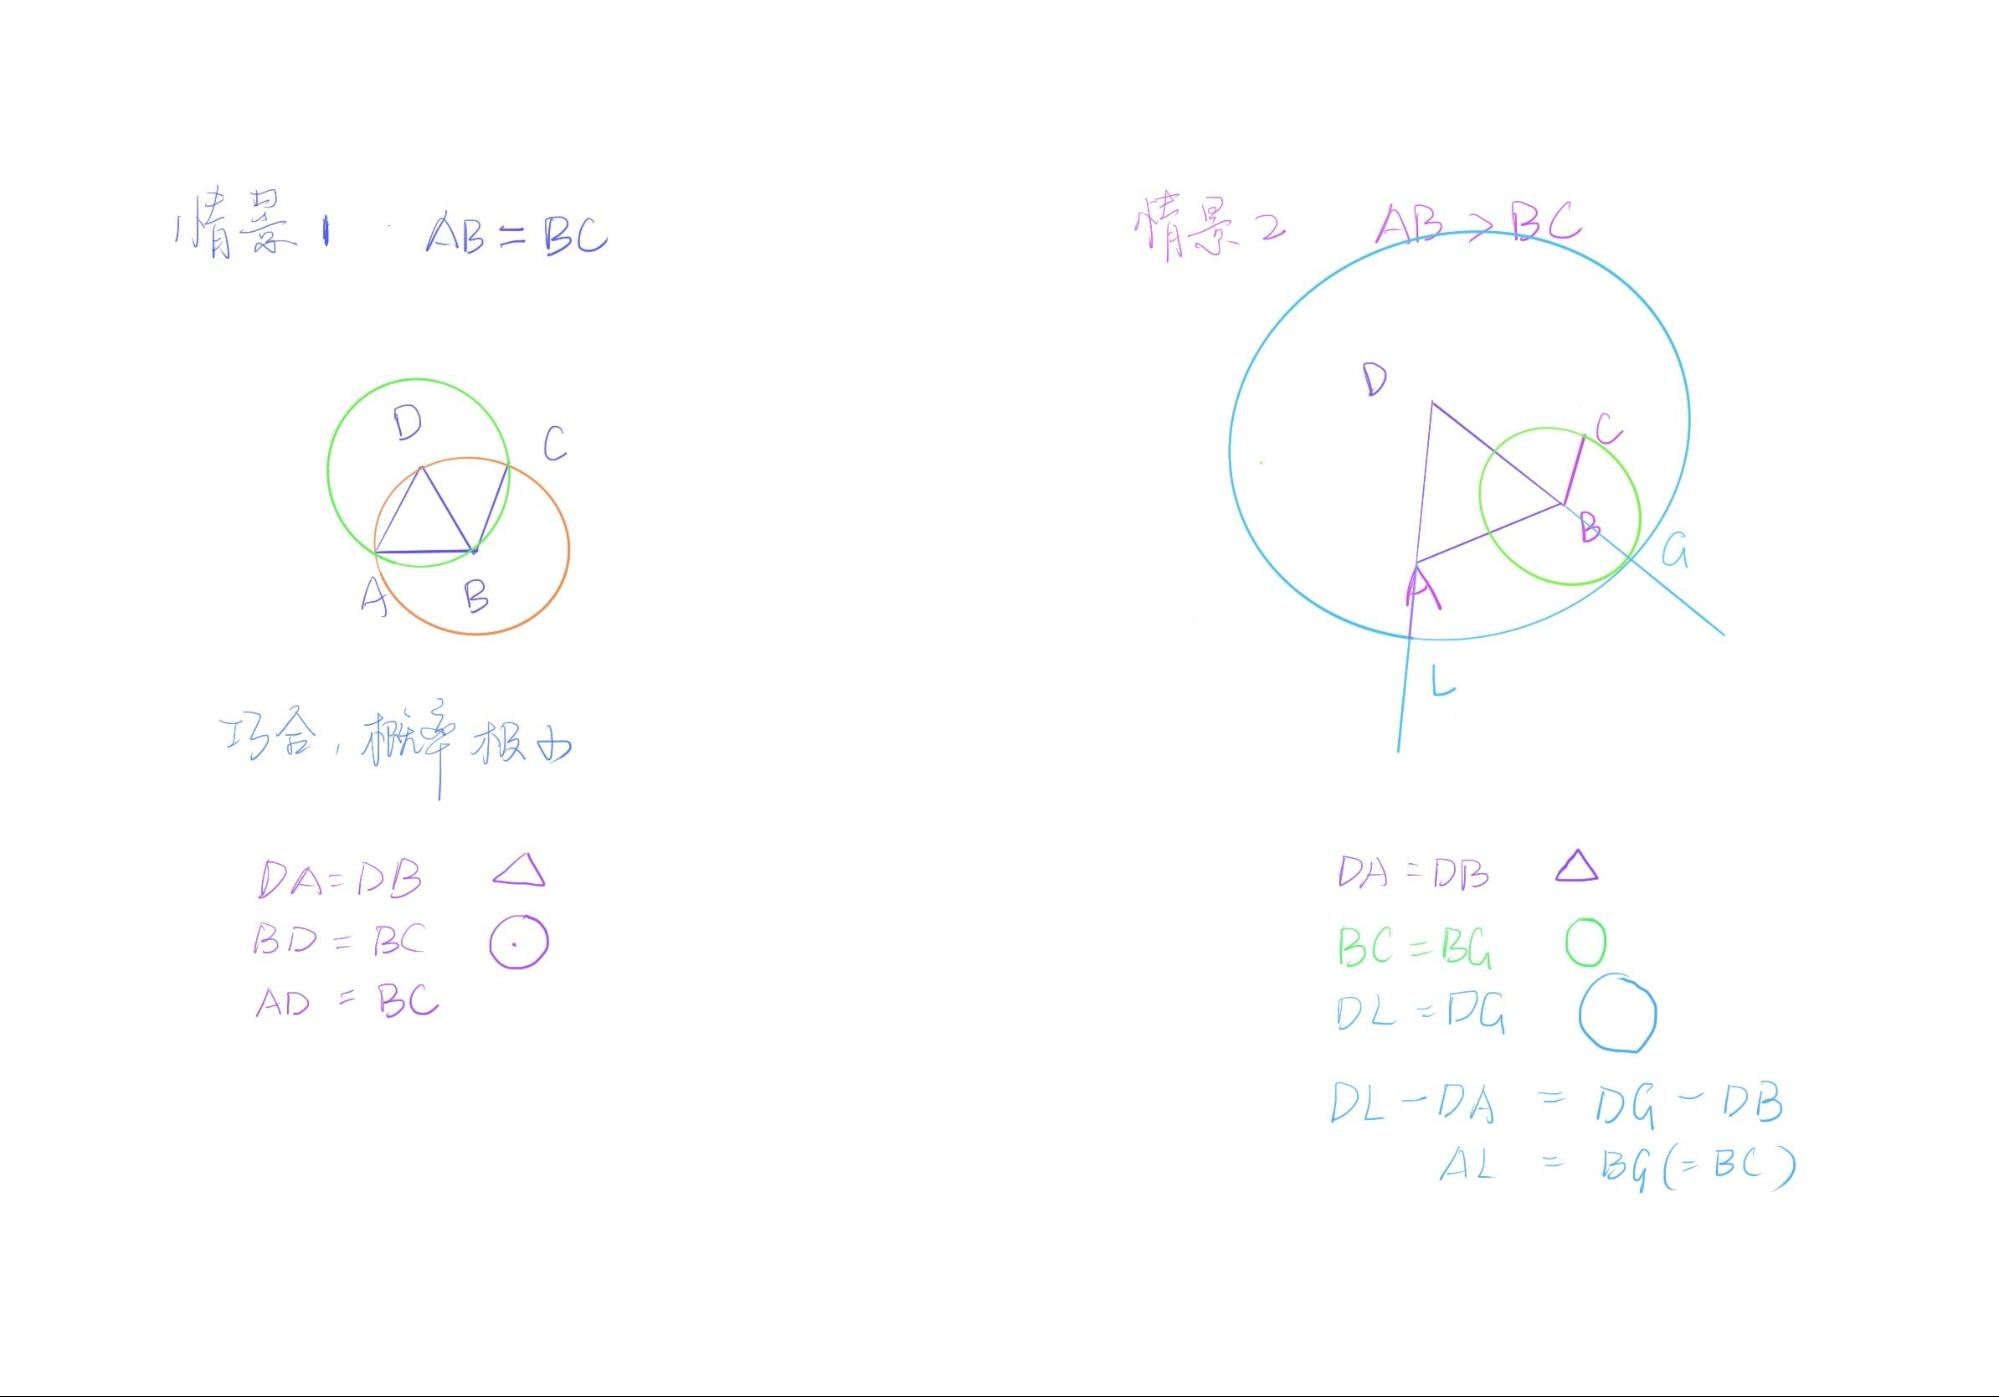
\includegraphics[width=1\linewidth]{./image/02-prop2-image1}

如果我们将三种情况用等式来标明,会发现量的大小也并没有影响逻辑推理。如此说来,图像传递了我们怎样的信息呢?

\textbf{相等(AB=BC)}
因为BC=BD,DB=DA,所以DA=BC
注意这里并不能直接写AB=BC

\textbf{AB \textgreater{} BC}
因为DL=DG, DA = DB, 所以AL(DL-DA) = BG(DG-DB)
又因为BG = BC
所以AL = BC

\textbf{AB \textless{} BC}
因为DL=DG, DA = DB, 所以AL(DL-DA) = BG(DG-DB)
又因为BG = BC
所以AL = BC

在此想要学习的第二个部分,是以命题二为例,说明如何记忆理解一个几何证明。看命题二的完整论证,是非常长的文字,在刚刚我们也转换成了公式,似乎事情变得更加明了,但是字母并不好记,如何才能将这个证明题完全掌握呢? 尽管我们刚刚总结了图像不能概括命题,然而图像在此却是记忆的一大助力。

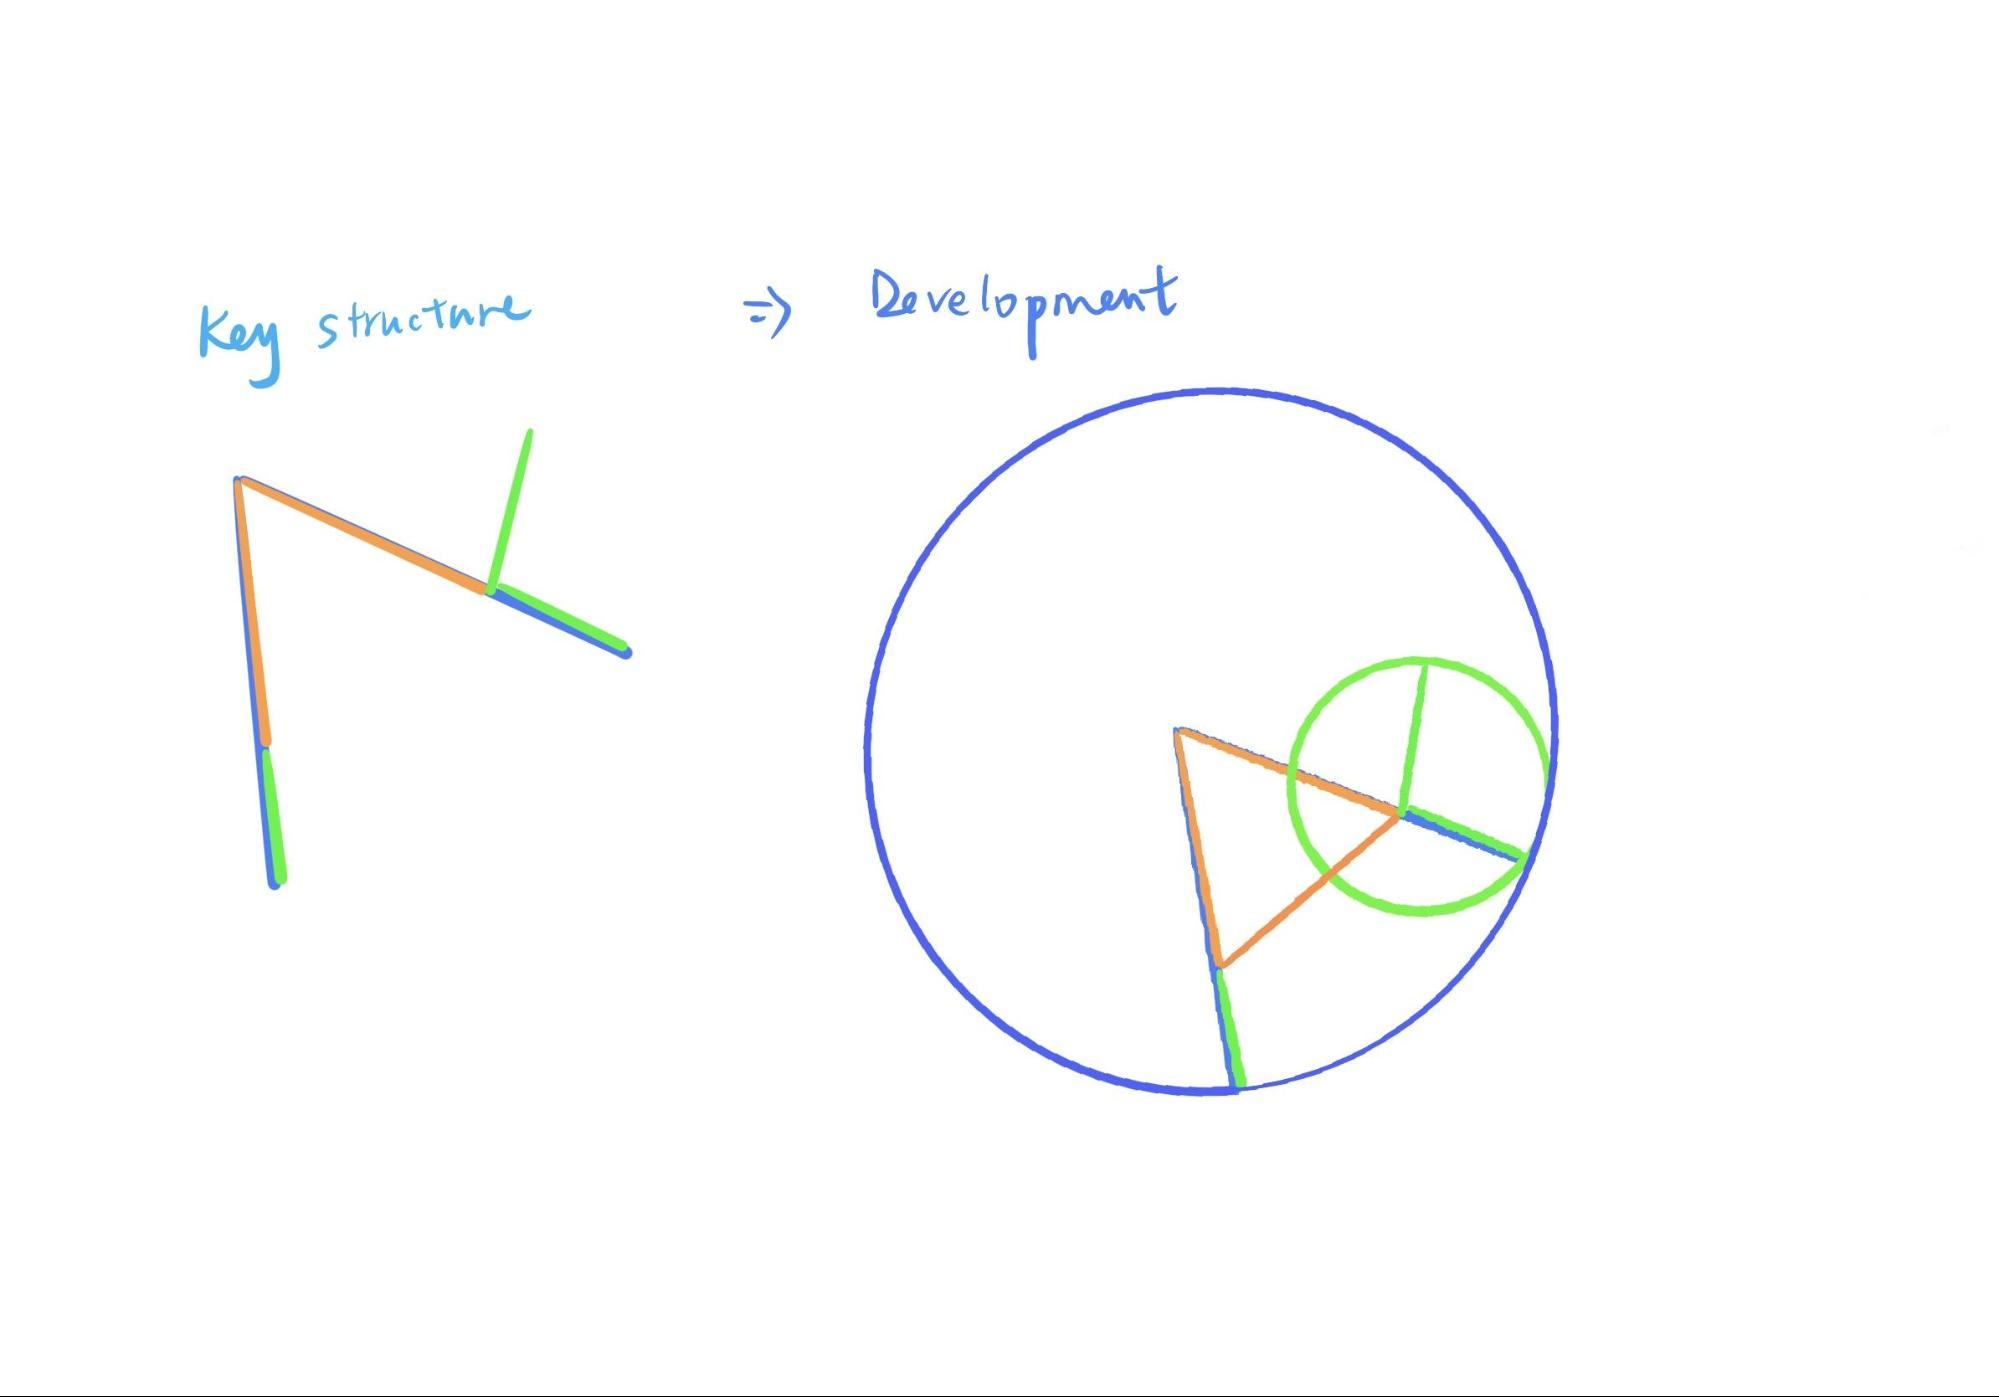
\includegraphics[width=1\linewidth]{./image/02-prop2-image2}

我们可以将完整的图形进行简化处理,只记最核心的部分,即两条边加旁边的小尾巴即可。之后想着两条边是某圆的半径,小尾巴和某边的一部分也是另一个圆的半径,此边的剩余部分和另外一条边的某部分是等边关系,所以另外一条边剩余的边和小尾巴相等。如此,通过色彩线段就可以回忆起整个命题的推理了。任意一道几何题,必定有其最核心的点和线,以及关键辅助线,而学习几何最重要的一部分也是学会抓重点和脉络,一旦能够通过图像把握证明的结构,那么整道题都会迎刃而解。

基于命题二就先讨论到这里了。

参考作业:

图像 与 文字

找一个绘本,随意找一页,尝试去定义文字和图像中重合的关键信息。只看文字,自己想象图画,然后只看图画,尝试自己用文字描述。

\hypertarget{ux7b2cux4e09ux8bfeux547dux9898ux4e09}{%
\chapter{第三课(命题三)}\label{ux7b2cux4e09ux8bfeux547dux9898ux4e09}}

\textbf{给定两条不等线段,从长的线段中截取一条线段,使等于短的线段。}

今天我们来看命题三,命题三非常短,然而今天我们讨论的内容就是如何去理解命题三的简短特征。

今天的讨论内容可以通过编程进行理解,而Alex在课外已经接触过编程,这无疑降低了理解上的难度。来看这个编程的例子。

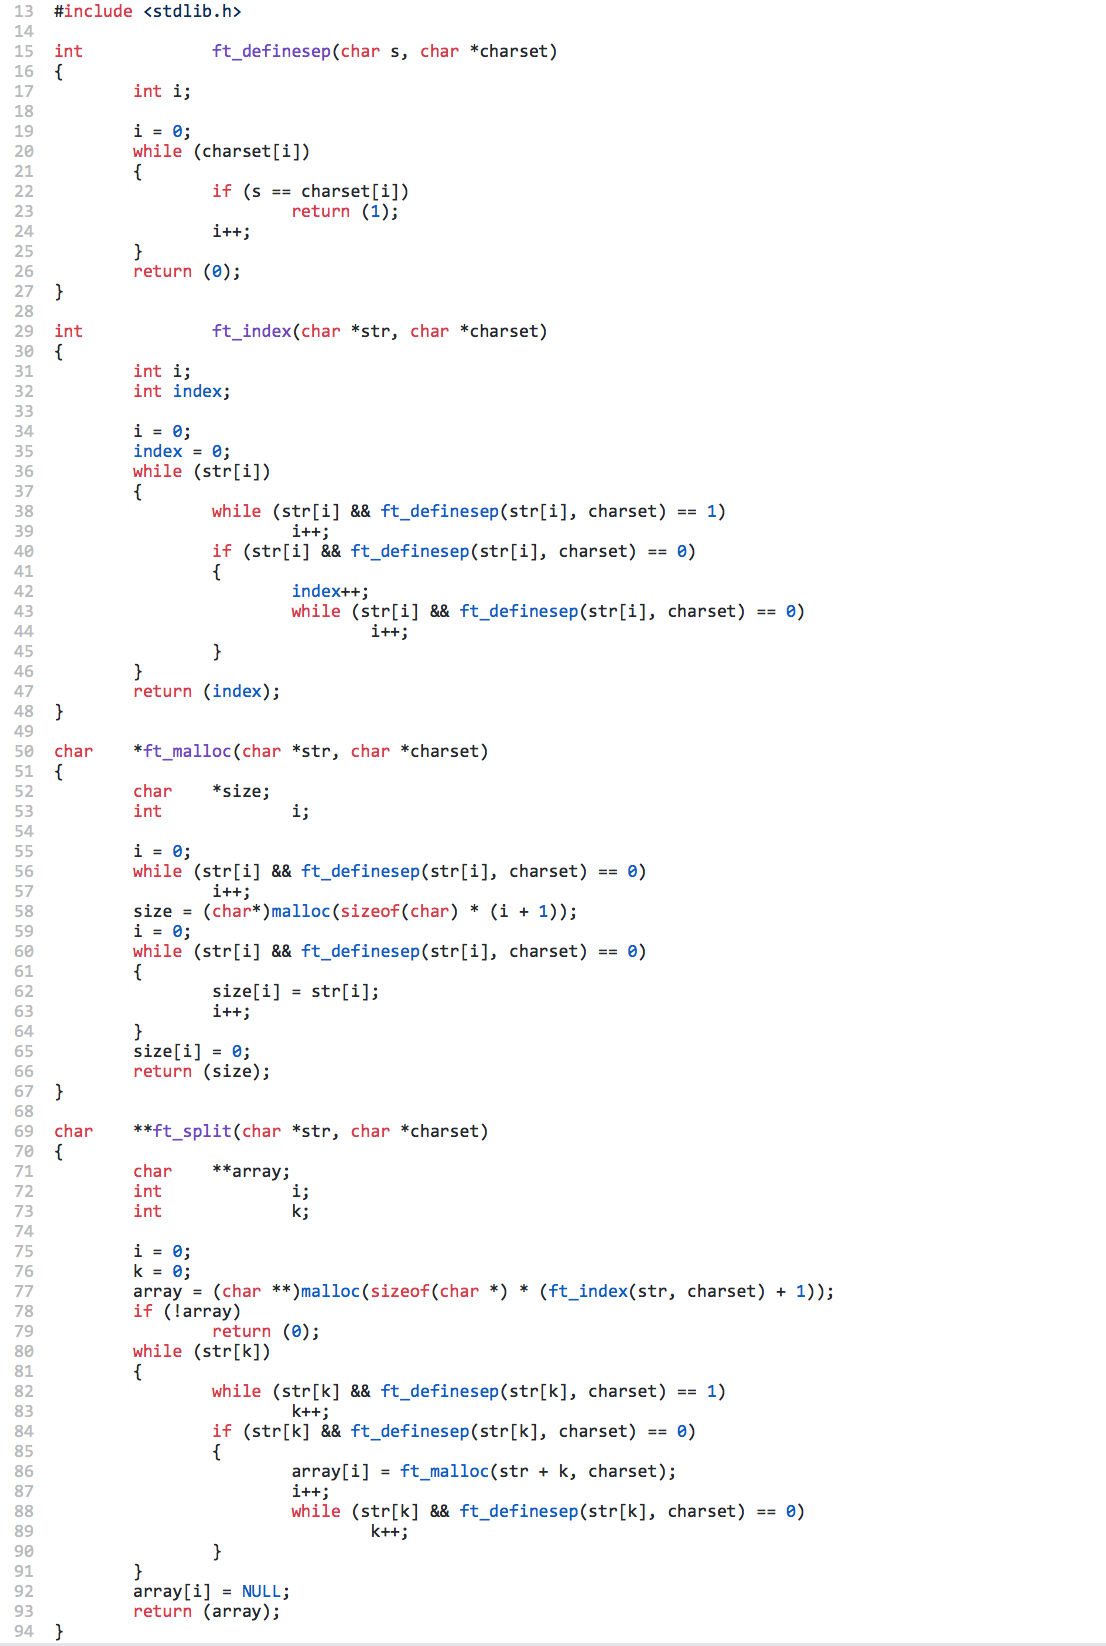
\includegraphics[width=1\linewidth]{./image/03-prop3-image3}

这个例子是用编程语言C语言写的,当然我们这节课的重点不是理解这个代码的内容,而会放在格式上面,并和欧几里得的命题三进行一个类比。

首先第一行有一个include stdlib,这是说在以下的代码中会调用到stdlib这个库当中的某个功能(是malloc),如果没有第一行的抬头,那么运行到malloc这一行代码的时候,就会报错,无法进行,因为与malloc相关的功能都无法调用。这个库对应在欧几里得的数学体系中其实就是证明之前的定义公理公设的集合,只不过C语言中有大量的定义,因为根据他们的功能性,将它们分组,只在用到的时候进行调用。

之后我们会看到四个独立的``循环'',其实前三个循环都是小循环,而最后一个char ft\_split才是主循环。现在我们观察这个代码,我们会发现这个顺序是不能够改变的。因为ft\_index引用了ft\_definesep, 然后*ft\_malloc引用了ft\_definesep,最后的ft\_split引用了前三者。如果改变任一顺序,代码都会报错,因为电脑线性地读取代码,如果运行到某一个''ft'',而这个''ft''在之前没有被定义,则电脑不能理解要做的内容就会报错。

欧几里得也是一样的道理,命题三之所以简短,是因为命题一二都已经提前预置好了。命题一二三放在同一页纸上,并且抬头写上包含定义公理和公设,这样才是一个可以完整运行的命题三。如果没有特意将命题一和二单独列出来,而是那么应该插入到命题三里面,参考如下:

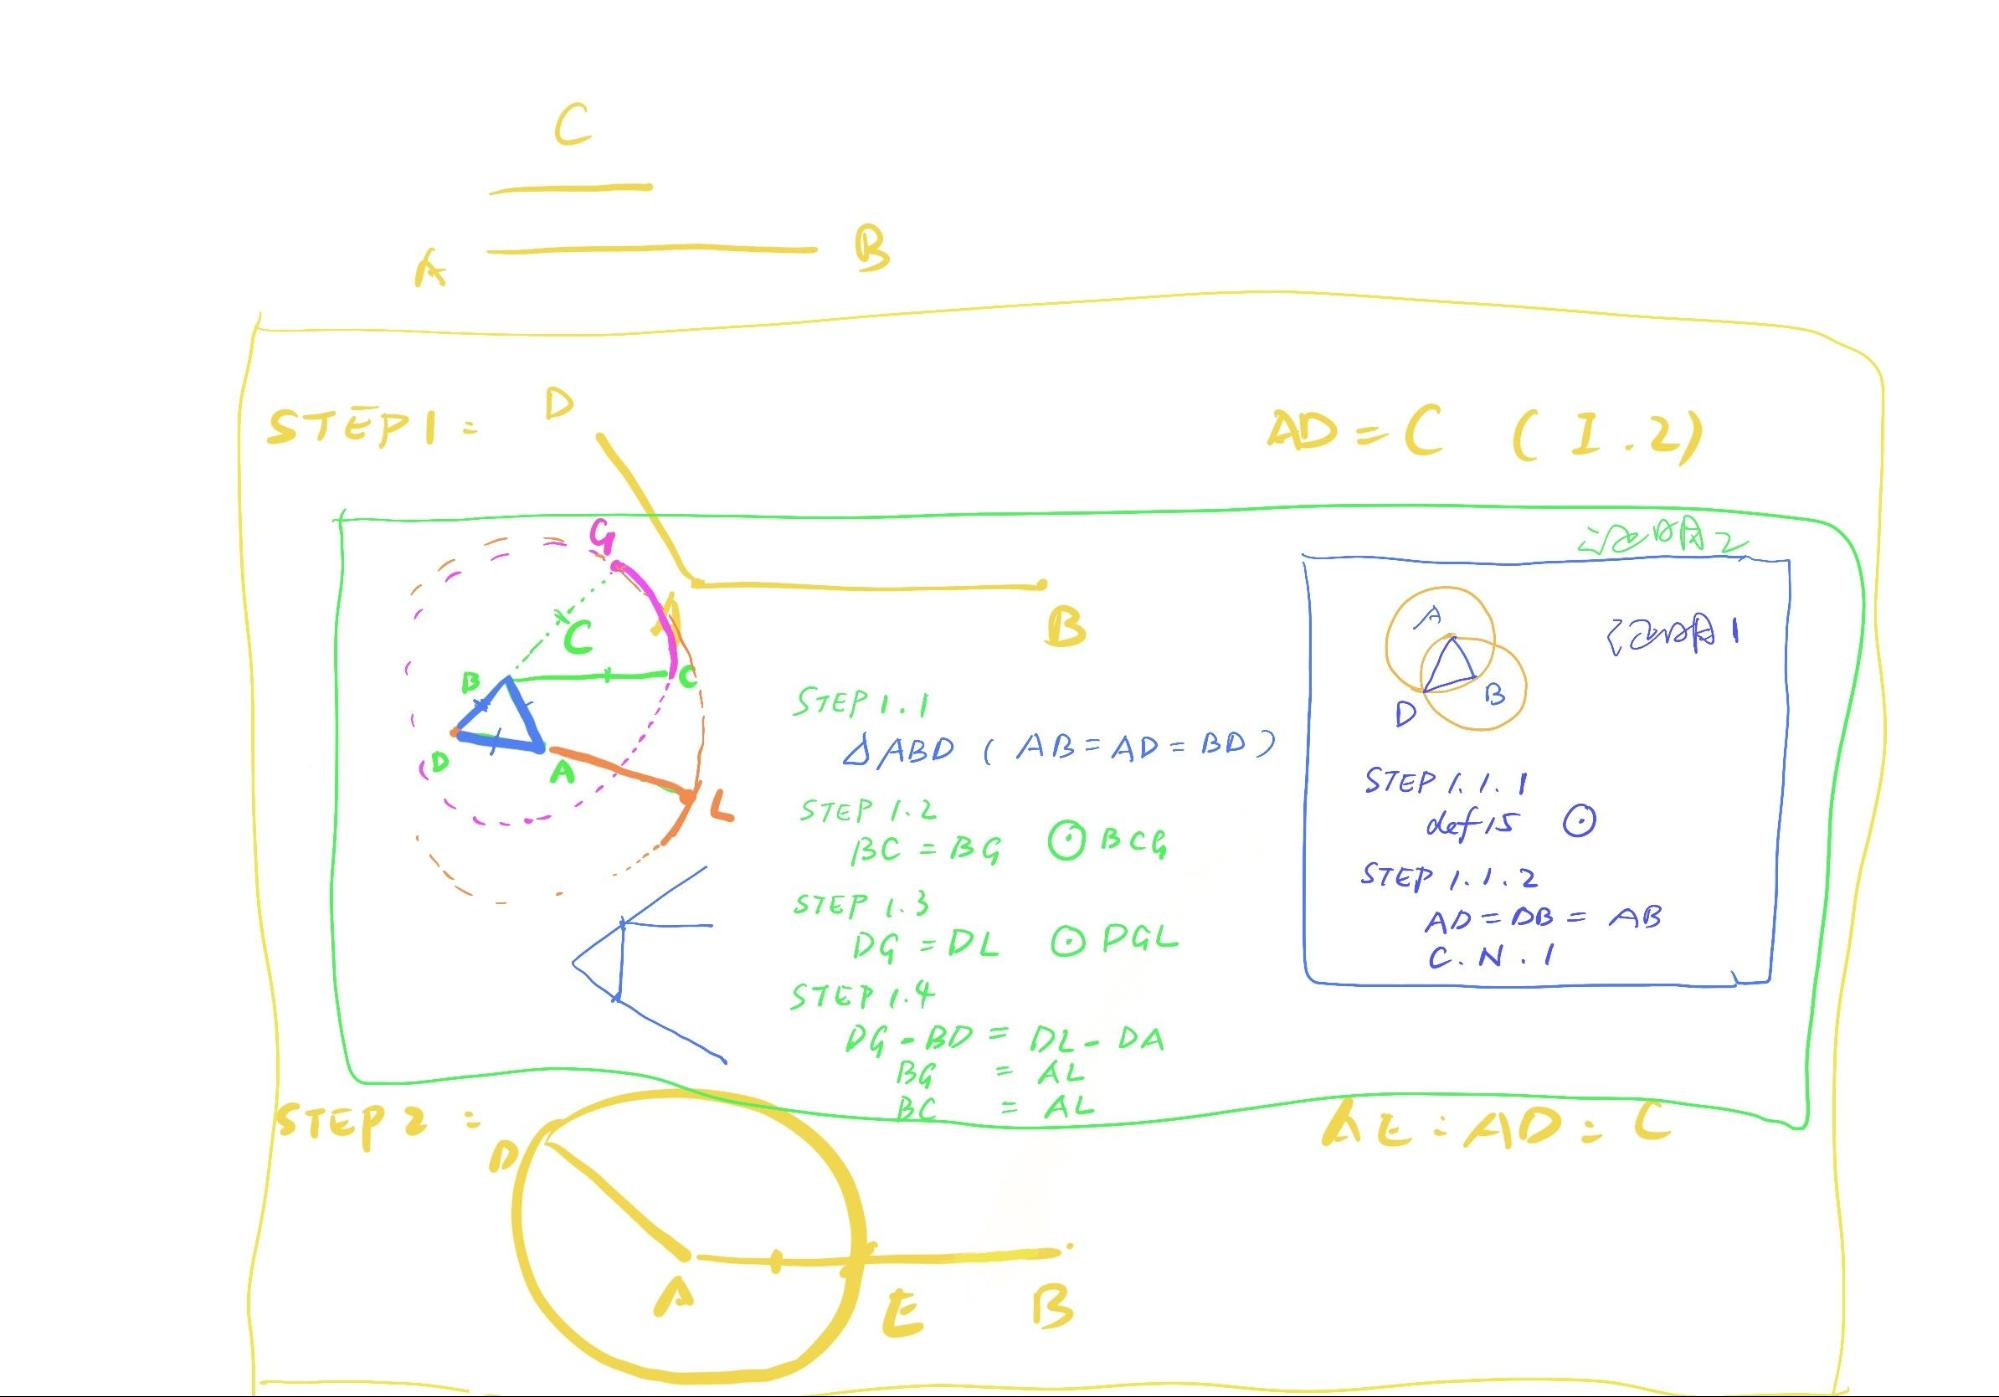
\includegraphics[width=1\linewidth]{./image/03-prop3-image4}

这里就会有一个很有意思的讨论,在什么样的情况下,一个模块要独立出来?这个问题等同于以下两种情况:在欧几里得的证明中,命题一和命题二为什么要单独出来呢?哪怕写进命题三里也并不会导致篇幅过长。在我们的代码案例中,为什么不能把小循环都写入大循环而是要单独出来,用的时候去调用呢。

对于会编程写代码的Alex来说,这个问题并不难理解。因为有几行代码太常用了,与其每次都要重复性的写几行,十几行,不如单独列出来,想用的时候一行命令调用即可。在欧几里得的命题证明中也是这个原则,如果我们判断一个某一个部分会经常被用到,那么我们就需要这个部分以先置命题的形式写出来,以方便后续的使用。欧几里得的《几何原本》这本书甚至可以被视为一本最初的编程代码全集。想想手动写几万行代码,全凭记忆调用各个命题,是不是就更能理解这本书对于那时时代的一个超越性?

下节课开始讲命题四,而命题1-3与命题四有一个很重要的区别。那就是前三道命题其实都是在``作图''、``绘制'',画三角形,画某个线段,截取某个线段。而命题四开始才是证明,那么下节课我们就来一起看欧几里得是怎么通过逻辑来证明事物的。

参考作业:

在日常工作中,有哪些可以提前进行的``分组''性质活动可以帮助到我们?
(这个问题的目的是引导学生思考他们的日常工作并提高其效率。例子。准备一周的衣服,以节省早上挑选的时间,买一周的牛奶,而不是每天都经过杂货店。)

\hypertarget{ux7b2cux56dbux8bfeux547dux9898ux56db}{%
\chapter{第四课(命题四)}\label{ux7b2cux56dbux8bfeux547dux9898ux56db}}

\textbf{如果两个三角形中两条边互等,并且这些互等的边所夹的角也相等,那么他们的底边也互等,三角形全等,剩余的等边所对的角也互等。}

今天我们一起来看一道非常有争议的命题,命题四。

Alex说这道命题讲的是全等三角形,数学课上已经学了。因此Alex直接口述证明。Alex的证明就是因为两边及夹角相等,所以两个三角形全等。那么我们的问题就来了:有没有想过为什么因为两个边相等夹角相等,所以两个三角形全等?这是全等三角形的一种判定方法没错,但是一开始它是怎么成为一个判定方法呢?我们现在就是探究数学课本为什么这么讲。要知道数学书这么写就是因为欧几里得最开始这么说了,但是欧几里德为什么这么说呢?同样的道理,我们也不能因为它是欧几里德,然后就直接相信他说的话,就直接觉得这是对的。我们也要仔细的看一遍这个证明题。命题四的特殊之处,就在于很多人看完这个全等三角形的证明,认为欧几里得的论证时有问题的。

Alex自己读完证明题,也就问出来了大家都会注意的到的问题,欧几里得为什么可以把一个点放到另一个点上面,又怎么能够保证两点重合又相等。在前面的公理中,欧几里得写了公理4:彼此重合的事物相等。这个公理4不如公设5讲平行的那条出名,然而在我眼中,它的意义却十分重大,因为这个公理是连接现实和几何世界的一座桥梁。重合是一个现实世界中的概念,它是没有在定义中出现的,我们是直接将一个现实中通用的概念,搬运到了几何世界中,然后与相等画了等号。命题四的蹊跷之处,也是源于此,它介于一种不真不假的状态,在现实和几何的交界处被描绘了出来。

Alex说如果可以移动和重合,那也可以旋转,在旋转的情况下,因为始终是同一个三角形,那么旧的和新的就一定全等。是的,也是可以的,那么在这种情况下,前面的公理就是讲重合,就需要描述旋转的性质了。另外Alex也提到了用尺子和量角器的方法,如果说旋转还在那个不真不假的两个世界交界处,那么用到尺子和量角器,就是完全站在现实世界了。这是不一样的。

这个证明题本身的内容,还有另外一个需要注意的地方,就是它本身逻辑的递进关系。证明题本身分成两部分:边角边证全等;全等证余边余角相等。第二部分常常被忽略掉,因为人们下意识的认为,两三角形全等,那么余边余角相等,但其实中间还有夹一步。那就是因为三角形重合,余边余角也重合,所以相等。这个相等不是从三角形的全等直接推出,而是也用了公理四的重合。

另外这道证明题只是关于边角边证全等的,并不涉及其余证全等的方法,比如边边角或者边边边。这一点需要特别注意,其余的方法仍然需要证明才能使用。

讲到这里,也就和Alex一起讨论了为什么数学课和数学书中,教的是定理和性质而不是证明了。其实也不难理解,从古到今,数学家们不停的发展这个学科,写了特别多本书,都是每个人一辈子思考的内容,而发展到今天,我们享受前人努力的成果的同时,也有一个问题,就是我们要在很短的时间内把这些内容都理解和吸收,之后才能继续发展。那这就要求将学习内容精炼和压缩。也就是将被广泛认可的基础证明当做定义告知。然后你就不需要知道他怎么证明,而只需要把它当做定义去使用,因为其他人已经替你证明了他是正确的。而这里的小弊端就是给你造成一种印象:这个东西可以直接用,他就是这个样子的。其实不是的,这些性质和定理在最开始也都是被证明出来的。比如两直线平行,同位角相等,就是命题二十八。所以,我和Alex说,希望他在学习数学的时候也多思考,存有一个怀疑态度,尽管百分之九十九点九九九,课本上的内容尽管不需要证明都是正确的,但是这种怀疑的态度可以保持你思维的敏锐性,多观察,常思考。就比如这个命题四的三角形全等,真的是百分之百正确么?Alex很快就意识到,这其实也不是的,只是因为这里是平面几何,在曲面上就是不同的样子,Alex画出了这样的例子(插图) ,而这种思考其实就是非欧几何的起源。

另外在这节课的证明论证中,Alex的表达方式也涉及到一个很有意思的问题,也就是数学三种不完整的表达方式:一种是文字描述。第二种是符号和字母。而第三种是图像。我问Alex觉不觉得这件事情非常有意思,就数学到底是什么?好像数学是一种东西,然后它可以用至少三种方式来表达。但是这三种方式表达的数学似乎都是不完整的。我们将这个疑惑留着,慢慢思考。

最后,在这节课上,Alex自己主动思考并且提出了接下来的上课方式。Alex需要课前预习证明题,在每节课开头,我会口述命题内容,Alex自己画图并且论证命题,可以自己想也可以用欧几里得的方法。在课前准备的时候,总要看一下欧几里得的方法,如果和自己的方法不一样,要思考一下哪里不一样,为什么欧几里得用了这种方法。

注:这个证明题用英文读的时候,有几个单词需要学习:enclosed; corresponding.

\begin{itemize}
\tightlist
\item
  enclosed: 围成的,en = in 表状态; closed 封闭的,封闭的状态也就是围起来的
\item
  corresponding:对应的, respond回应;co相互,一起;相互回应也就是一一对应
\item
  另外还有熟悉let\ldots.(已知条件)I say(证明结果)的格式
\end{itemize}

参考作业:

\begin{itemize}
\tightlist
\item
  数学是创造的还是发现的,为什么?(不着急回答)
\item
  找到一个用符号表达的数学方程的例子,用图像/实际产品来描述它,用数字来应用这个原理。你觉得哪种方式更合适?
\item
  看看你自己的例子,或者拿 ``a+b,1+1,一个苹果和一个橙子''来说,对你来说,哪个更容易接受,为什么?这是否告诉你一些关于数学的来源?
\end{itemize}

\hypertarget{ux7b2cux4e94ux8bfeux547dux9898ux4e94}{%
\chapter{第五课(命题五)}\label{ux7b2cux4e94ux8bfeux547dux9898ux4e94}}

\textbf{在等腰三角形中,两底角互等,并且如果两腰继续延伸,底边下的两角也互等。}

今天的命题五是关于等腰三角形的,通过命题五的学习,我们将更进一步理解欧几里得证明的严谨性。在反思平常数学的局限的时候,我们寻找避开思维陷阱和突破的方法。

命题五是证明等腰三角形两底角相等,且将两边延长之后,底角的补角也相等。

Alex很是有趣,他说等腰三角形底角相等,直线角180度各自减去相等的两底角肯定也相等呀。所以Alex的尝试一总结为:将命题直接当成性质用,不经证明即声明相等,然后推论补角相等。为什么会发生这样的情况呢?因为Alex记的是等腰三角形两腰相等,两底角相等。这对他来说是类似定义一样的存在,不需要证真,是合理存在的。这也是数学课本中的一个比较普遍的问题,将原本需要证明的命题全都当做了``定义''教授,学生很少去思考为什么和这是怎么证明出来的。

启发学生去反思这个问题,也并不难,只需要提醒一句,在已知的条件中,我们只知道有一个三角形,并且两边相等,其余的一概不知。再问一下他是怎么知道两底角相等的,自然Alex就开始了第二轮探索,尝试自行证明两底角相等。Alex的尝试二可以总结为希望借助等腰三角形三线合一的性质来证小三角形的全等,然后证底角相等。我再次提醒他,三线合一的性质也是需要证明的,我们目前并不知道这一点。于是我们开始分别看三种情况,来推导底角相等。

首先我们一起看了角平分线的可能性。如果能够将角平分,那么等腰三角形被角平分线所切割成的两个小三角形可以通过SAS(边角边)判定全等,那么两个底角作为全等三角形中对应的部分,也自然而然就是相等的了。但是这里有一个问题,我们如何知道所画的直线可以将顶角平分?在Alex的演证过程中,我需要反复问的就是,为什么这条直线将角分成了两半?我同意所画直线将角分成了两部分,但是我怎么知道这两部分是相等的呢?你是不是也需要先证明然后才应用。也就是说,可以用角平分线的方法,但是也要先证明所画的线有将角平分的功能。

我们可以一起来看一下角平分线这个例子

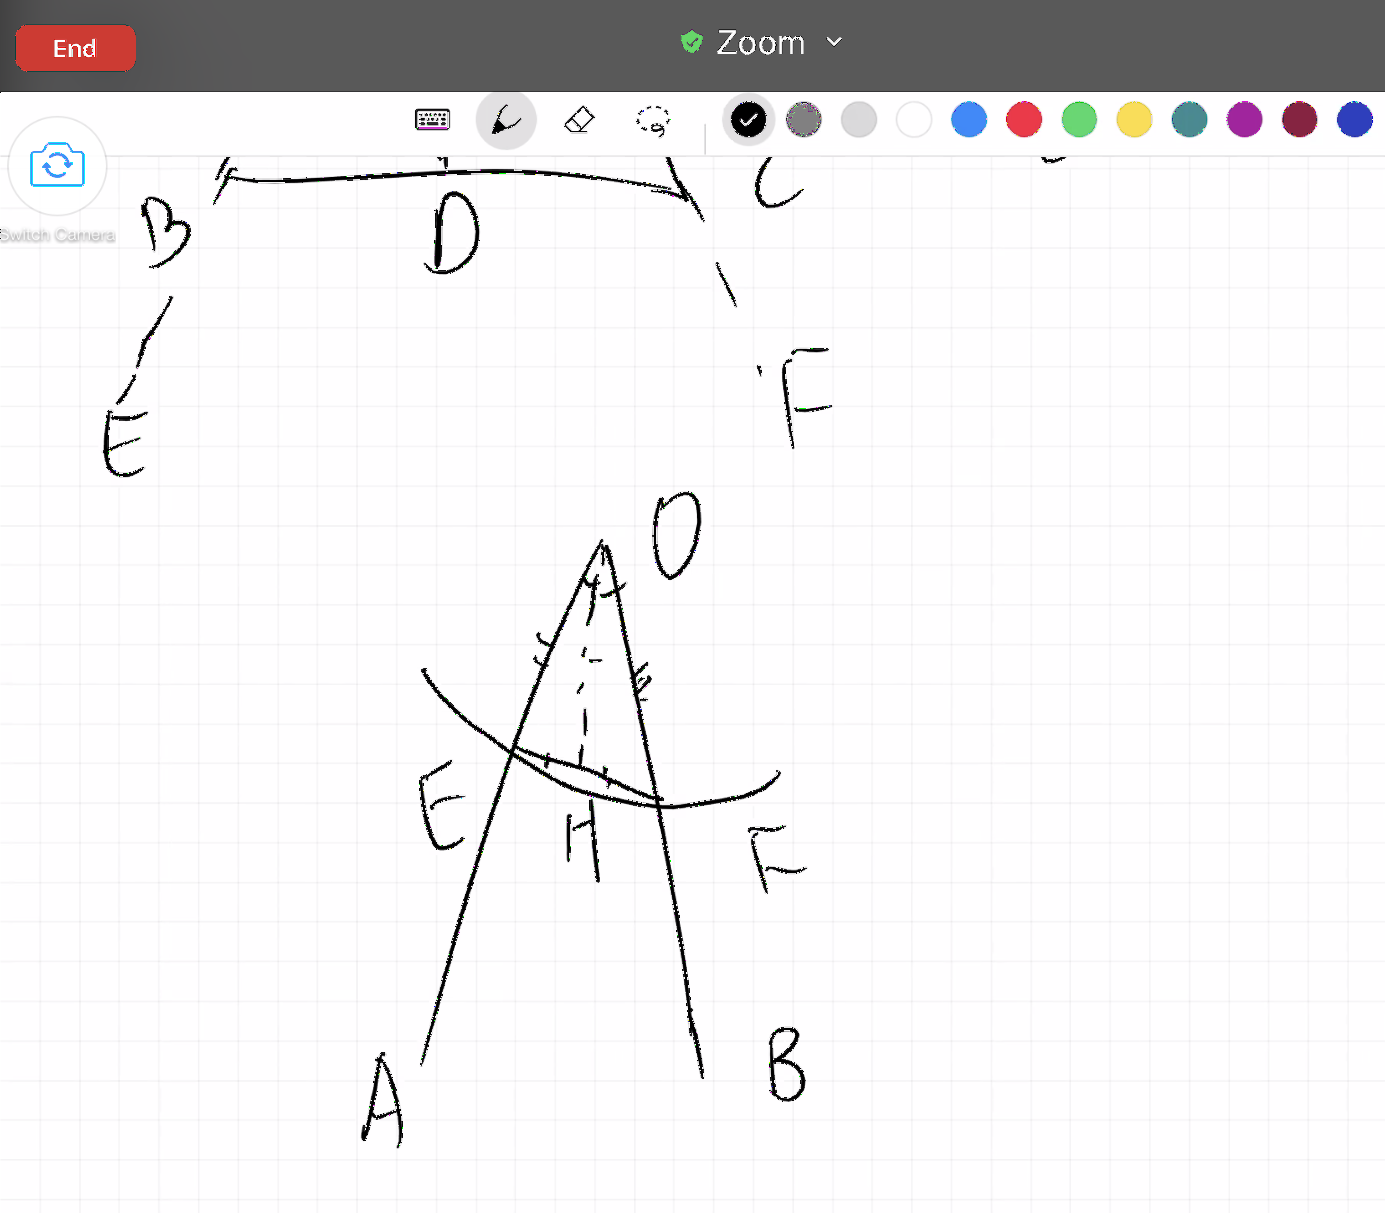
\includegraphics[width=1\linewidth]{./image/05-prop5-image7}

所以我们发现如果要用到角平分线,则需要通过SSS(边边边)的方式证三角形全等,而SSS证全等在这一步并不是一个已证明的命题,尽管在命题四的学习中,我们已经对全等三角形有了最初步的认识,但是我们只是知道了两件事情:

\begin{enumerate}
\def\labelenumi{\arabic{enumi}.}
\tightlist
\item
  SAS(边角边)可以证明两三角形全等
\item
  全等的三角形三边三角各自相等
\end{enumerate}

从以上两项中是无法直接推导出三边证全等的,也因此Alex不能顺着证明角平分线。

其实无论是第一次对命题的尝试性证明,还是这里的角平分线解法,背后都是同一个问题,那就是学生将学校数学课堂学到的直接运用,而没有去思考背后的逻辑和证明。凡是被老师教授的,在课堂上学到的都是理所当然的。而这一课最重要的学习,也不是欧几里得的证明方法,而是改变之前的反射弧,形成新的习惯,多退回几步问几个为什么。

Alex之后也尝试了画中线还有垂直线的方法。画中线似乎也很简单,在底边上取中点,然后连接顶点即可,但是是不是也需要证明所取的点恰好将底边分成了相等的两部分?而垂直线,我们会发现SSA(边边角)是不能证全等的。和Alex一起看了一组边边角相等但三角形不全等的反例。

只有将种种自己的想法都一一尝试过后,才能更好的理解欧几里得所选用方法的精妙。也因此在学习的过程中,很值得鼓励去自行尝试解题。

除了证明的方法,对这道题的理解,还有一个捷径。也就是用实践的方法来说明等腰三角形底角相等的性质,虽然这不是严谨的证明,但是可以给我们信心,也可以让我坚持对这个性质的探寻。举个例子,最简单的就是说有一个等腰三角形,我们将它对折,然后就发现两部分完全重合,那么底角自然是相等的。Alex也想了一个方法,是有一个直角三角形,然后将它的一个直边固定住,然后旋转180度,原本的三角形和新的三角形组成的大三角形就是等腰三角形,且底角必定也相等。逻辑证明和生活的重合与不同也就这样展现在了我们的面前。数学本身是一种连接,它在成就当下的同时,也为将来的推论做准备,永远都处于一种承前启后的位置上,而生活很多时候不需要解释,不需要逻辑,眼睛看到的,耳朵听到的就是真实。

再一起看完命题五之后,我们一起浏览了一下命题九,因为Alex想知道欧几里得怎么画的角平分线。而我们发现这其中用到了三边相等证全等这一步。这就是命题八的内容,(命题四只证了SAS全等。)而命题八又建立在七上面等等,以此类推,最初的每道证明题都和后面的发展息息相关。忽然在这里,Alex也明白了全等三角形的性质也是需要证明的,并不是理所当然的。

参考作业:

\begin{itemize}
\tightlist
\item
  有没有什么常见的说法是别人没有证据就相信的?(不考虑宗教的。)你也相信吗?(看看推理对你的理解有什么影响)
\item
  把你上学需要的物品列一个清单。
\item
  如果下雨,这有什么不同吗?
\item
  如果在早上,你发现自己生病了,这有什么区别吗?
\item
  条件是如何影响清单的?(要看到晴天可能是开始时的一个隐藏的、未经证实的假设,它影响了决策过程)
\end{itemize}

\hypertarget{ux7b2cux516dux8bfeux547dux9898ux516dux4e03}{%
\chapter{第六课(命题六\&七)}\label{ux7b2cux516dux8bfeux547dux9898ux516dux4e03}}

\hypertarget{ux547dux9898ux516d}{%
\section{命题六}\label{ux547dux9898ux516d}}

\textbf{如果三角形中两角互等,那么两角各自对应的边也互等。}

命题六的内容是证明等角对等边。这道题用的是归谬法,也就是反证法,通过否定等角对边不等的这个可能性来反向证明等角必对等边。而之前的证明题都是正向顺序证明。就好像是材料和模型,之前的证明题是把材料一点点把最后的模型搭起来,而这道证明题是拆模型,看能不能拆出和预期不同的材料。这里比较有意思的是,我们反思自己的接受度,和Alex一起讨论了是否两种方法一样的令人信服。

对于Alex来说,无论是正向的证明还是反向的证明,只要在步骤上逻辑没有问题,他就是可以接受的。对我而言,我可能会下意识的先想一下为什么不能正向证明,是只可以反向来说服么?我也邀请Alex尝试不用归谬法,而是正向顺序的尝试一下证这道题,我们画图思考但并没有找到完全合适的思路。Alex提出用特殊证明法,将等腰三角形设定为直角等腰三角形,然后通过计算sin45度的方法来说明两边相等。虽然这个方法在这里``超纲'',但至少说明了Alex对在学校学习内容的活学活用。

我们没有找到合适的几何思路并不能说明这道题是完全不可以通过正向来证明的,但至少正向证明是困难的,而归谬在这里更易理解。

那么如果一定要用归谬法的话,有什么需要注意的呢?大概就是归谬,在归的时候,要适用于各种情况,将所有其它可能性都否定,这样才会给我们剩下所希望得到的唯一解。

\hypertarget{ux547dux9898ux4e03}{%
\section{命题七}\label{ux547dux9898ux4e03}}

\textbf{在同一条直线(由它的两端点),构建会在同一点相交的给定两线段,那在同一条直线上(由两端点),在同一侧,不能构建出交于另一点的另两条线段,使之与之前的两线段相等,即分别到每个端点的线段。}

命题七的命题说明有些绕,但用白话解释一下,是说在一个线段的一侧任意找一点,不能找到第二个点使得连接线段两端点后的新的线段长度相等。

这里的方法还是归谬法,命题内容并不难理解,和Alex很快的一起复盘了欧几里得证明的过程。在这里值得记录的是Alex提出的自己的归谬方法,是运用了运动轨迹和画圆的方法来说明的,记录如下:

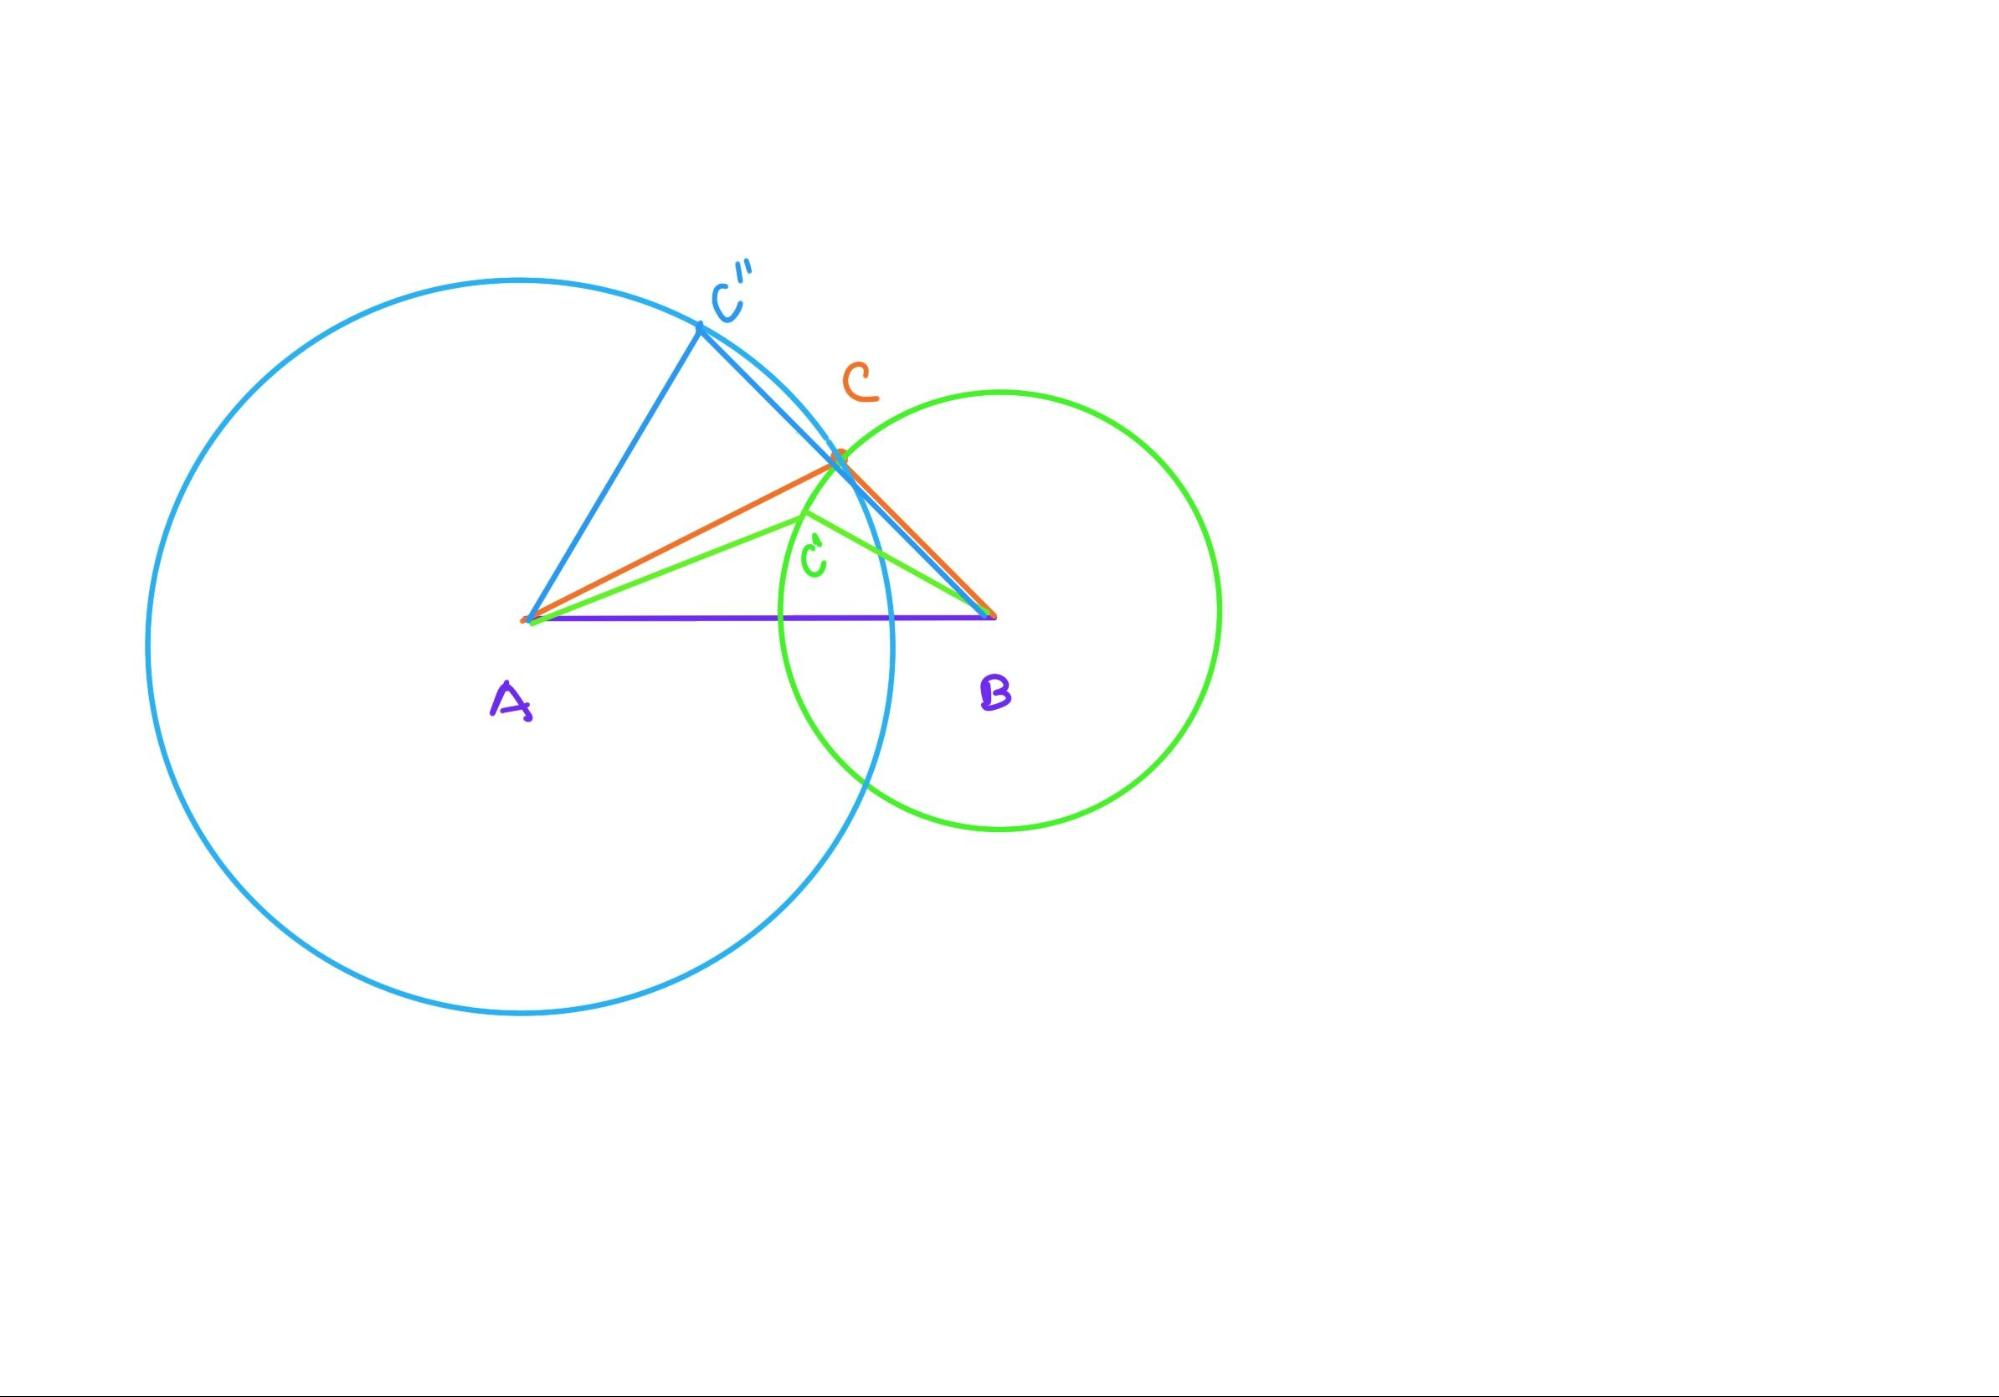
\includegraphics[width=1\linewidth]{./image/06-prop7-image6}

以A为圆心,AC为距离画圆;以B为圆心,BC为半径画圆。若BC距离保持不变,C点必须在圆弧上移动,任意其它一点与A的距离必定会发生变化,或大或小,因为圆A与圆B在AB的同一侧只有一个交点。同理若保持AC距离不变,则BC距离发生变化。因此在AB的同一侧找不到第二个点使得AC,BC保持不变。

Alex的这个证明方法是以运动的角度解题,思路十分的开阔,同时Alex在证这道证明题的时候也提到了,如果能找到第二个点使得所连的线段都相等,那么就是在三维空间上,而不是在一个平面上。也就是说Alex已经注意到了这些命题没有言说的先天条件,``平面''几何。

学到这个命题,很容易就会发出疑问,为什么我们需要这个命题呢?似乎看不到一个明确的目的。根据我们以前和编程内容进行比较的学习,不难推测,欧几里得是在为之后的命题证明做铺垫。只是不明确是为证明什么而做准备。其实在生活中也是这样的,有些事情可能看起来在当下是没有意义的,但是其实是之后生活的一部分。通过学习这些命题,至少会帮助我们理解两件事情:一个是拆解;而另一个是准备。将大的任务拆解细化到可以完成的层次,有些准备任务可能在当下是看不到意义的。

参考作业:

\begin{itemize}
\tightlist
\item
  介绍数独的游戏,试玩,同时思考有没有用到归谬并且这个策略是如何发挥作用的。
\end{itemize}

\hypertarget{ux7b2cux4e03ux8bfeux547dux9898ux516bux5230ux5341ux4e00}{%
\chapter{第七课(命题八到十一)}\label{ux7b2cux4e03ux8bfeux547dux9898ux516bux5230ux5341ux4e00}}

随着Alex对欧几里得证明的熟悉,也因为证明形式的重复性,在内容的学习上,我们会略微加快一点速度。这节课我们讨论命题八到十,以及快速浏览命题十一。

\hypertarget{ux547dux9898ux516b}{%
\section{命题八}\label{ux547dux9898ux516b}}

\textbf{如果两个三角形分别有两边各自对应相等,并且底边也互等,那么被等边夹的角也互等。}

Alex首先尝试自己证明,在第一次尝试中,Alex选用了等腰三角形,这里有一个在题意理解上的误区,读题读的不够仔细。题中的两个三角形两边各自对应相等,这里并不是等腰三角形,而是说有两个三角形的边对应相等,欧几里得试图证明的是一个通用的定理。

(绿色,等腰三角形的特殊情况;紫色,一般通用情况,可以是锐角/钝角/直角/等腰/等边三角形等等)

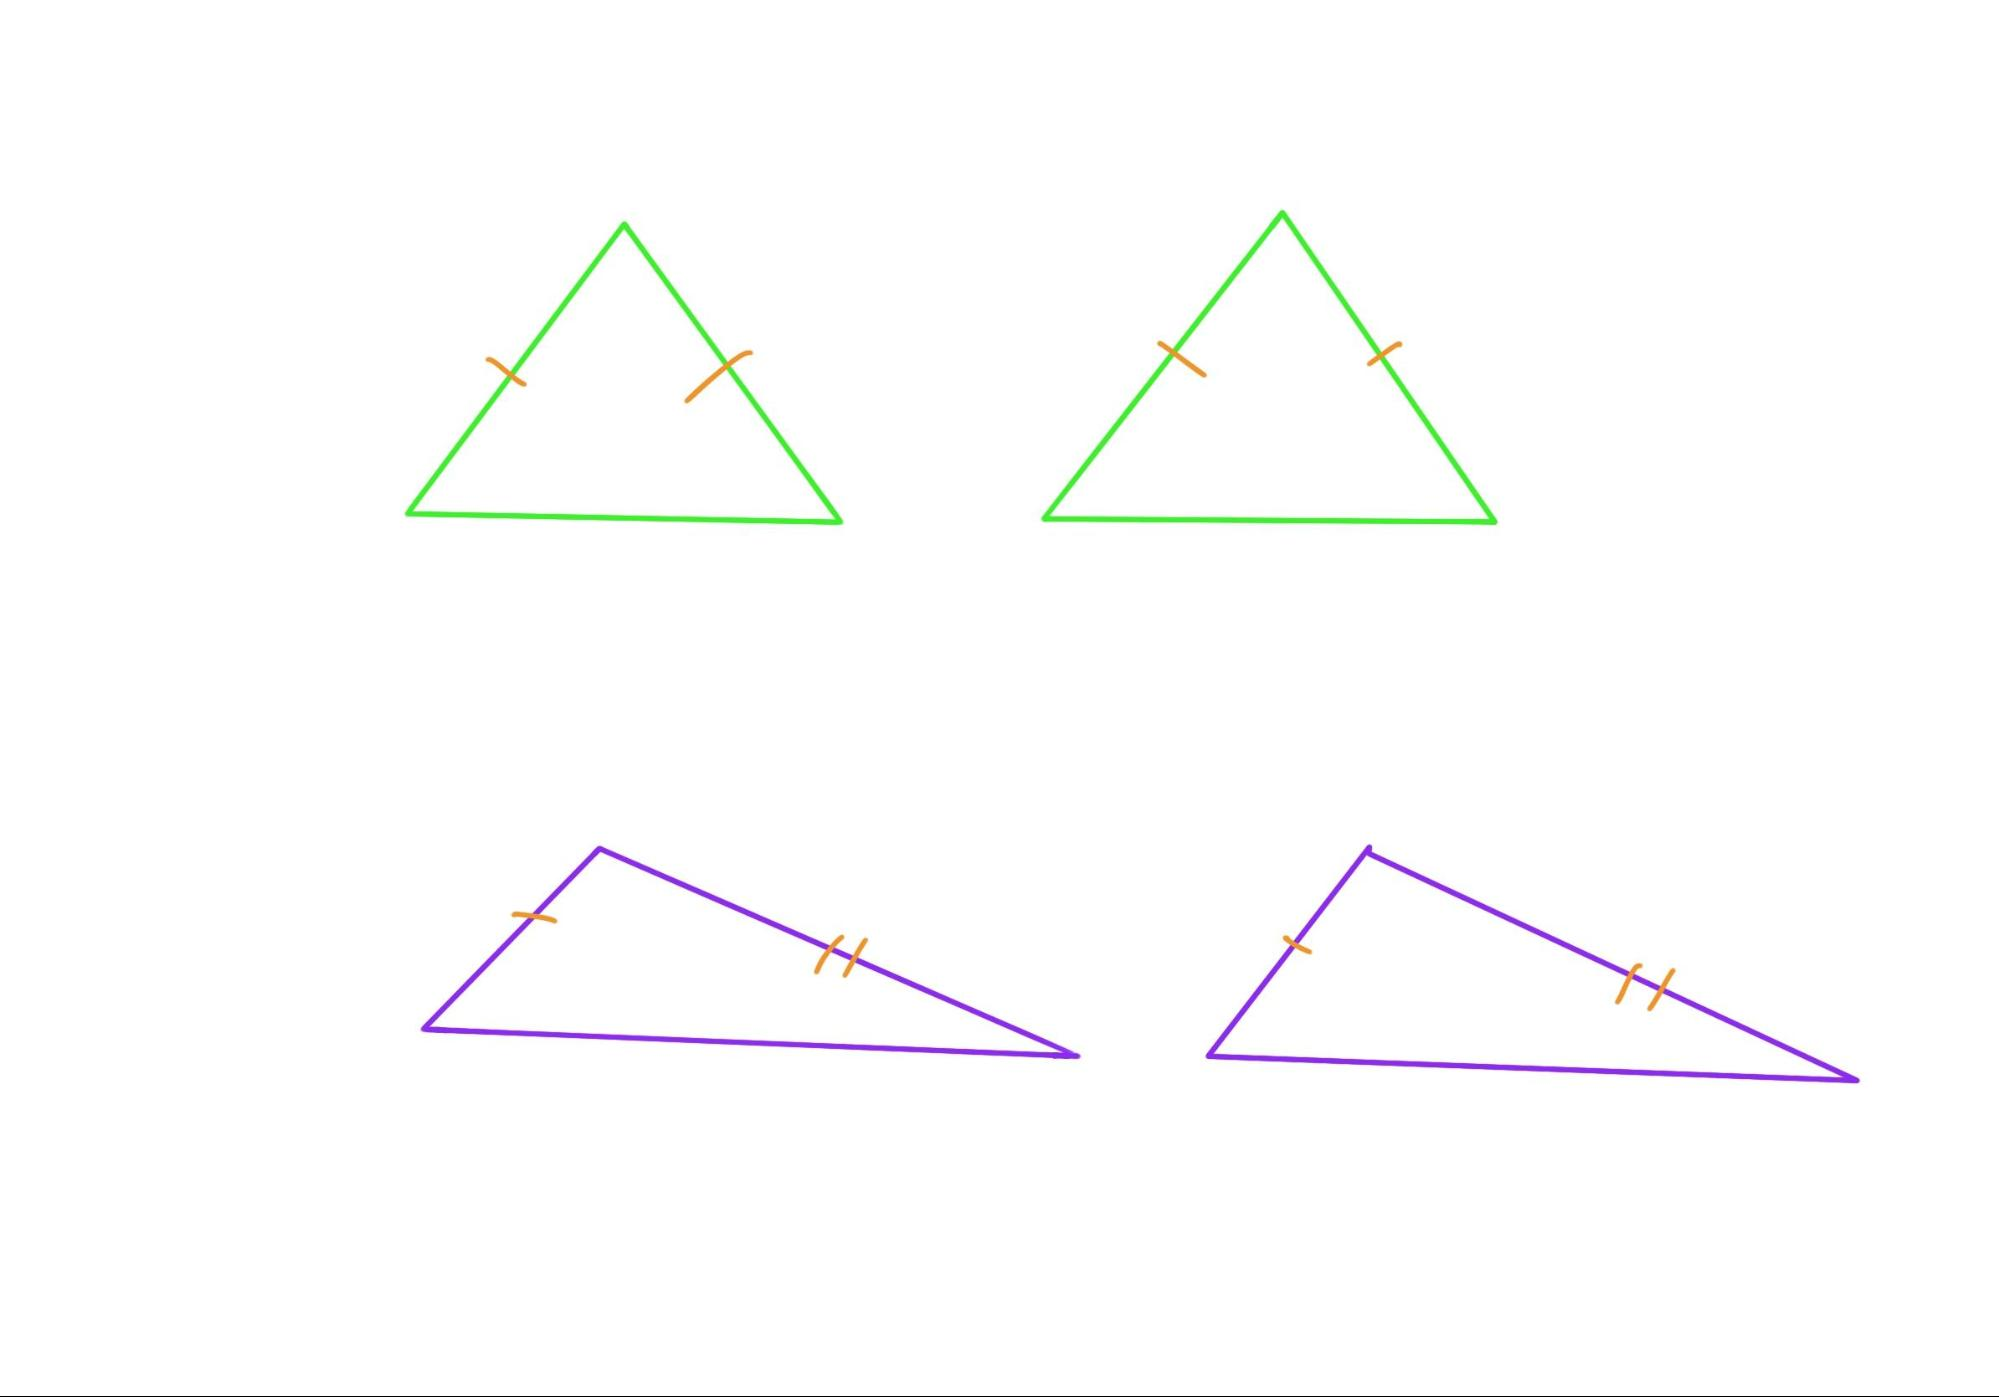
\includegraphics[width=1\linewidth]{./image/07-prop8-image9}

由于命题七是命题八的一部分,并在推理中发挥了关键作用。

正如昨天预料到了,今天一起看完命题八,Alex说这才懂了命题七的存在。

\hypertarget{ux547dux9898ux4e5d}{%
\section{命题九}\label{ux547dux9898ux4e5d}}

\textbf{将给定的直线角平分。}

命题九是画角平分线,之前的课上粗略的看过,今天要求Alex再仔细地证明一边,我们会发现这道题的逻辑框架是这样的:等腰三角形,等边三角形,全等三角形=\textgreater 角平分线,此命题的实现需要三层铺垫。等腰三角形的两腰相等,等边三角形的两条边,最后连线的公共边,最后一同构造了全等三角形的边边边相等的条件。

这道既短又简单的命题,其实还向我们展现了做辅助线技巧。辅助线是数学几何题解题的钥匙,画对了辅助线,几何证明也就很顺畅。有时候觉得辅助线是需要多尝试才能找到正确的一条,但是如果能够明确辅助线的目的,也是可以用逆序思维推理找到正确的辅助线的。比如命题九这个例子,题目的最终目的是将一个任意角平分。自然而然会让人联想到两个被平分的角各自是某两个三角形的一部分,通过全等可以推断对应两夹角相等。那么为了构造全等三角形,除了平分线这条共同的边,还需要等边和等腰三角形来搭建对应边相等的已知条件。如此,辅助线是关于等边等腰三角形的,而我们需要用辅助线将它们画出来。在数学几何练习题中,对辅助线一筹莫展的时候,不妨从结论倒着推,看需要什么额外的图像,那些额外的定理和性质来辅助证明,如此辅助线也就被找到了。

这道题讨论关于平分的概念,我们可以回到定义十七看一看那里发生了什么。

\begin{quote}
定义十七:任意一条穿过圆心,并两边都在圆周上终结的直线被称为圆的直径,并且直径将圆一分为二。
\end{quote}

定义十七说直径将圆一分为二,这个地方是不是平分?为什么欧几里得没有证明?对,他直接就这样说了,圆一分为二,这就平分的。我让Alex想一下为什么圆的平分就不需要证明。Alex说直径画了两个直线角,都是180度,所以两部分一样。那怎么证明那两个圆弧是一样的?这里默认了等角对等弧。那为什么等腰三角形里,等角对等边需要证明呢?

Alex的``割圆术''

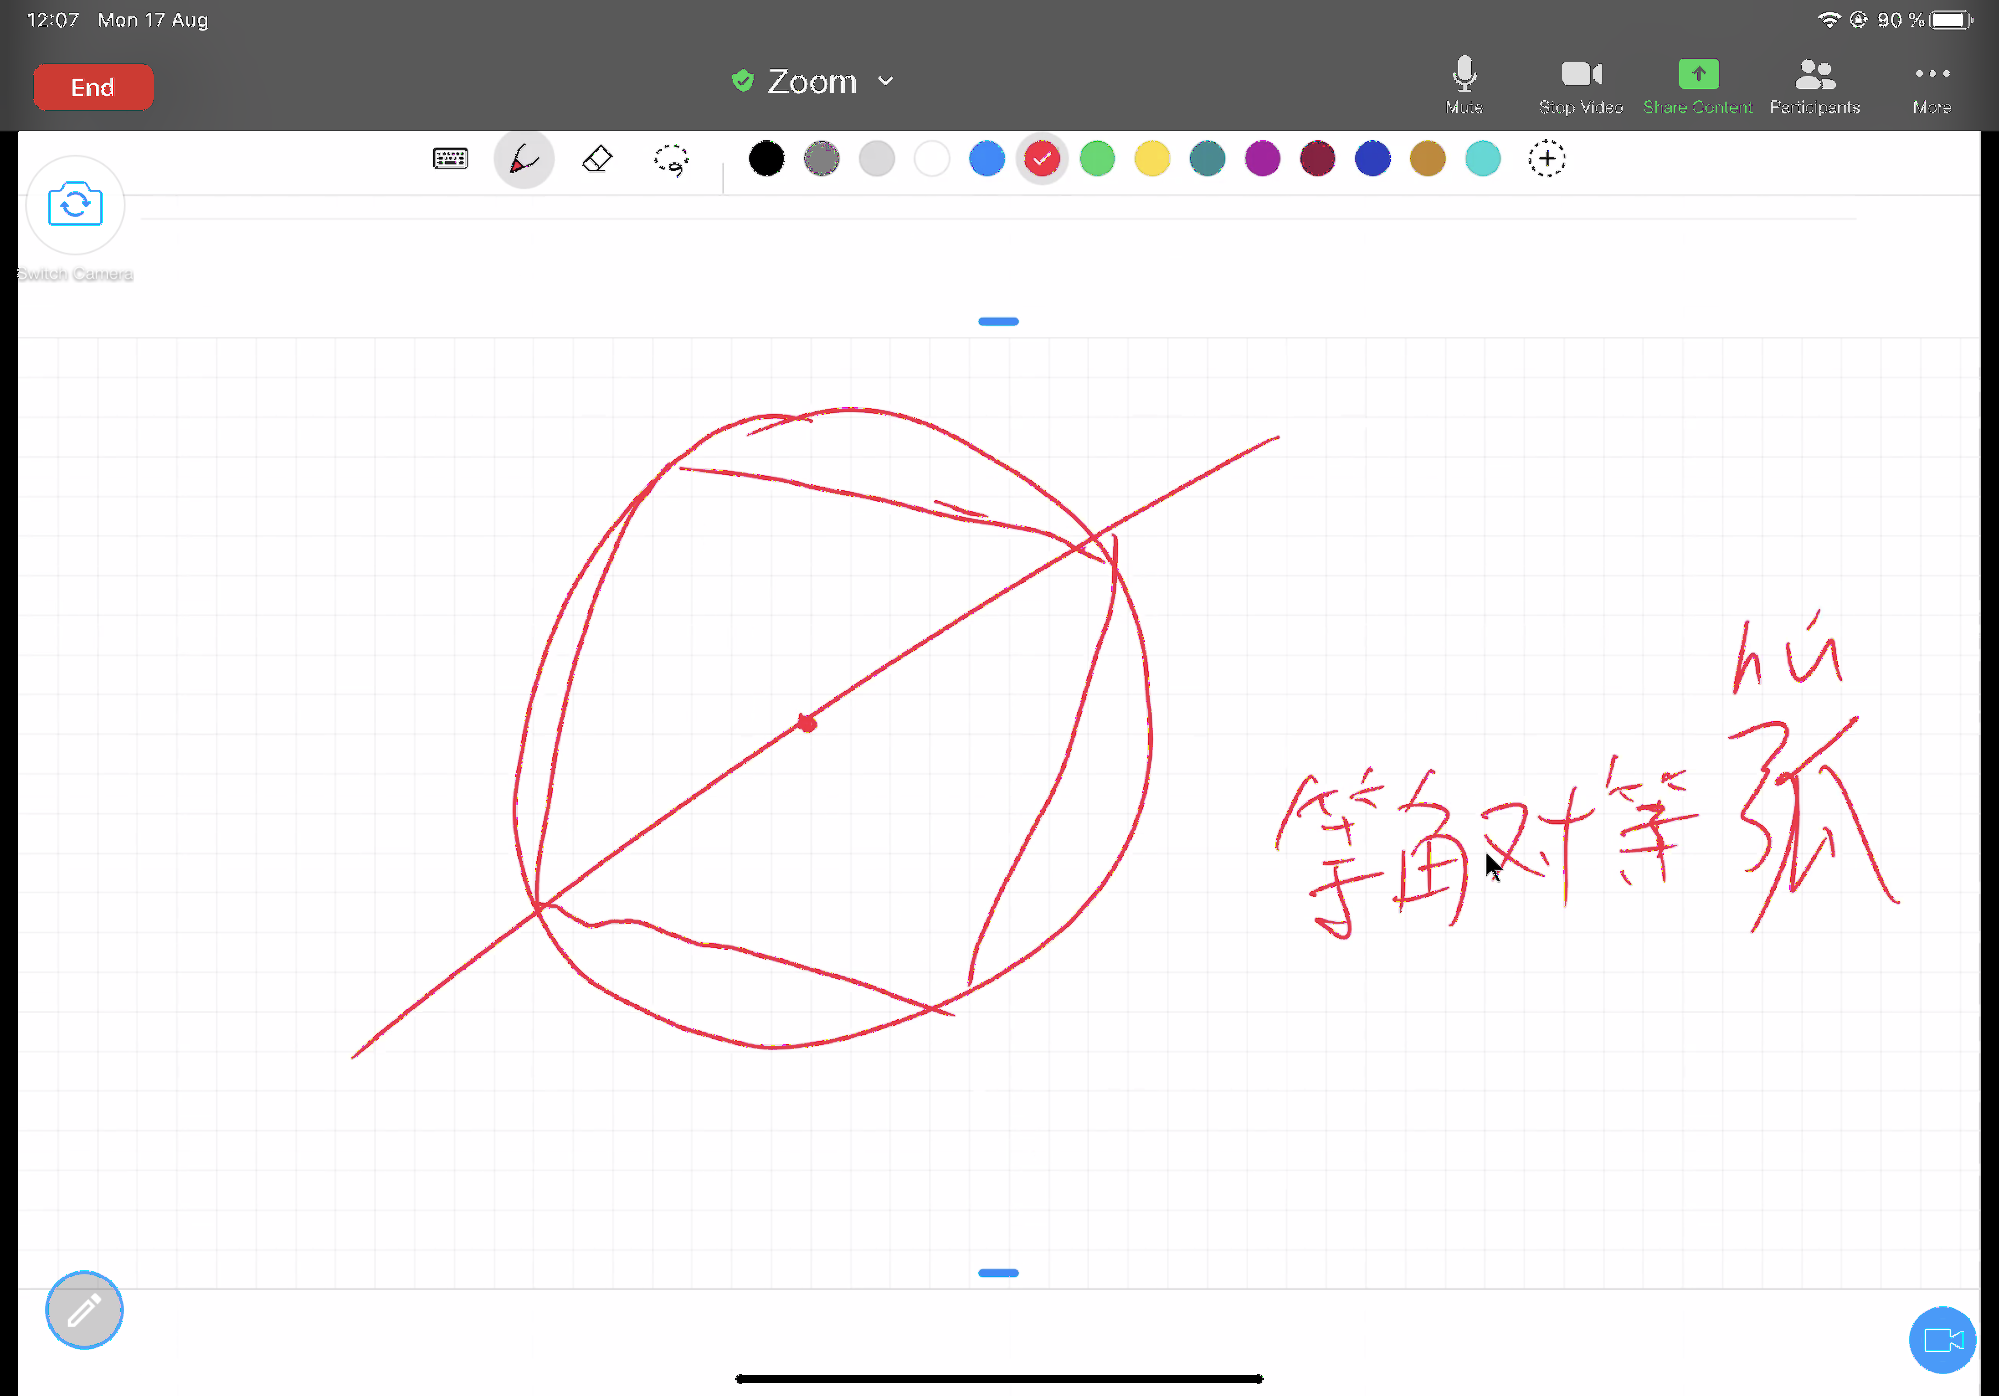
\includegraphics[width=1\linewidth]{./image/07-prop9-image8}
\#\# 命题十
\textbf{将给定的线段平分。}

命题十我们简单的过了一遍,这道题是命题九的延续,一样通过全等三角形倒推线段的平分,并没有难度。另外这也是俗称的等腰三角形三线合一性质的一部分,在这里是角平分线和底边的长度平分线重合了。

\hypertarget{ux547dux9898ux5341ux4e00}{%
\section{命题十一}\label{ux547dux9898ux5341ux4e00}}

\textbf{在给定直线的给定点上,画一直线与给定直线呈直角。}

其实做题上课也能看出孩子的性格,像是Alex,反而越难越有挑战性的题目更能调动他的积极性。简单的题目比较喜欢一带而过。像这道题,也是受数学课的影响,Alex会直接画垂线,然而我们其实还没有证出怎么画垂线。这道证明题本身也是以上两道题关于``三线合一''性质的延续,这里是承接上一道题平分线段的连线,再证明在等边三角形中,同时也是能画的直角的线。因此,这里的顺序是:角平分线=\textgreater 中线=\textgreater 垂线。

数学的几何题,确实思路很重要,有了思路,基本上一道题也就解完了,但是表达也一样重要,因为哪怕是百分百完成的事情,最后的表达如果只呈现了百分之五十,那么在最后的沟通中,也就只有百分之五十。被省略的部分是不被认可的。下节课开始,我应该和Alex在不跳步骤,遵循格式的情况下重新再看一遍这道题,审视这个思路架构和他的表达。

\hypertarget{ux7b2cux516bux8bfeux547dux9898ux5341ux4e00ux5230ux5341ux4e09}{%
\chapter{第八课(命题十一到十三)}\label{ux7b2cux516bux8bfeux547dux9898ux5341ux4e00ux5230ux5341ux4e09}}

\hypertarget{ux590dux4e60ux547dux9898ux5341ux4e00}{%
\section{复习命题十一}\label{ux590dux4e60ux547dux9898ux5341ux4e00}}

\textbf{在给定直线的给定点上,画一直线与给定直线呈直角。}

上节课命题十一过得非常快,这里我们先复习一下,在这一次的证明中,我们关注一下欧几里得写证明题的格式。

命题序号:命题十一

抽象的命题内容:在给定直线的给定点上,画一直线与给定直线呈直角。

将命题内容翻译成具体的图像和字母符号,也就是将命题转化成接下来证明会呈现的内容:
- 设AB为给定直线,且C是其上一给定点。
- 所以要求从点C画一直线与直线AB呈直角。

在具体的图像和符号上的作图和结论:
- 在AC上设任意一点D;作CE使等于CD;【I.3】在DE上构建等边三角形FDE,【I.1】并且连接FC;我说直线FC与给定的直线AB呈直角且起于给定点C。

具体的证明内容:
- 因为DC等于CE,并且CF是公有的,两边DC,CF各自与两边EC,CF互等;且底边DF等于底边FE;所以角DCF等于角ECF; 【I.8】且他们是相邻角。
- 但当一条直线置于另一条直线上,并使得两个相邻角互等,每个角都是直角;【定义十】所以DCF,FCE都是直角。

证完的声明:
- 所以在给定直线AB的给定点C上作的直线CF与AB呈直角。
- Q.E.F.

你会发现欧几里得不是一边画图一边写证明,而是先画图,后证明,是分开的。这说明什么呢?说明《几何原本》这本书里的证明题,他不是对证明过程的简单展示,而是一个证明之后的归纳和整理。就好像是我们写证明题有时候需要一个草稿,最后试卷上写定稿一样,《几何原本》的证明题只是呈现给你了一个定稿。所以有时候我们说他思维缜密,前后连接的非常好,但也未必是从一开始就做到的,也有可能是逐渐补充完善的。它最后完善起来的这个格式非常值得借鉴:

首先每一个命题有一个序号数字能简单的代表它,然后是言简意赅的总结性内容。在证明开始之后,则是先将不易理解的抽象内容通过图像文字符号具象化,然后描述作图构建的步骤,接下来在完整的图像上回到原点,开始证明。证明完成后有声明来标注它的完成。你看它的格式是有始有终的,非常清楚。这种方式特别适用于与人沟通的写作,哪怕不是一道证明题而是一个实验报告,你都可以用这个形式来呈现你的作品,如果是一个报告,那就是以下的模样:

\begin{itemize}
\tightlist
\item
  标题、日期(作者)
\item
  报告概述(对标题进行进一步的解释,包括概念、方法论等等)
\item
  将概念性的问题实践化,描述相关的实验设备、背景,将实验和报告的主题联系在一起
\item
  重要的实验步骤和结果
\item
  具体的实验过程
\item
  最后将实验回归到报告的主题上
\end{itemize}

这种格式充分考虑了读者的接受度,从主题,概览,到具象化问题,到问题步骤和小结,一应俱全。这个格式运用的思路可以借鉴到不同的报告类文件写作中,这种方式未必呈现一个思考的过程,然而对读者友好,非常的系统化,可读性高。与之相对的就是散文一类的写作,或者由问题出发的探讨,往往这一类写作方式可以呈现作者的思考过程,但是也很容易将读者带偏。在写作的时候,要参考写作对象和目的来选择相应的方式。像数学科学这样的学科,都是带有普遍化目的写作,因而清晰的写作格式和架构就尤为重要;而文学类,更多的是侧重个体经验的描写,从细节处与读者共情,读者接受的不是同样的环境,而是所传递的情感,思考和个体反应,那么格式和架构就不是表达的重点了。

\hypertarget{ux547dux9898ux5341ux4e8c}{%
\section{命题十二}\label{ux547dux9898ux5341ux4e8c}}

\textbf{给定一无限直线,在线外一给定点上,画垂线。}

命题十二和命题十一是紧密相连的,看起来也有些相似,因而也让我们奇怪,为什么这两个命题不能合放在一起证明?我最开始也以为这里是直角和垂线的递进关系,但后来发现用另一种方式来观察更好:如果仔细阅读两道证明题的表达,会发现在条件中还是略有不同的。命题十一,谈论的还是线上一点,而命题十二,将范围延伸到了线外一点。也就是说,命题十一还在研习``三线合一''的性质之内,还需要借助等边三角形,而命题十二中的垂线则已经走出了三角形顶角/底边的范围, 可以是任意的线外一点与线的关系。

\hypertarget{ux547dux9898ux5341ux4e09}{%
\section{命题十三}\label{ux547dux9898ux5341ux4e09}}

\textbf{如果将一条直线置于另一条直线上成夹角,要么成两直角,要么与两直角相等。}

对于这道命题,Alex最大的困惑就是,一条直线不管和另外一个条线相交是否成夹角,它本身都应该是180度么,即两个直角,为什么还需要这样证明。

这个困惑需要被拆解成两部分:

第一部分是:无论我们用两个直角还是180度描述它,事实上我们想表达的都是一条直线与另一条直线所夹成的角之和不变。而且似乎这个道理从图像上来看是不言自明的。这么说是没错的,所以在这道命题中,我们需要一个度量办法将这个固定的量描述出来。这道命题不仅仅是证明这里有一个等量,而且还要以恰当的方式来表述这个等量,也就是第二部分需要解释的:为什么是用两个直角来表达,而不是180度。

从这门课一开始,Alex学习的一大障碍就是对数的执着。``两个直角''与``180度''这两个概念之间究竟有什么区别?在Alex的眼里,``两个直角''和``180度''指代的都是同一个图像,从这个角度来说,确实是如此的,都是第一部分中所提到的夹角之和,是个等量。然而这两个概念不同的地方在于他们的计量单位是不一样的。``两个直角''是直角乘以2,而``180度''是1度乘以180。我们在定义中有了直角的概念,然而在没有量角器的情况下是没有1度的,也没有180度。也就是说``180度''在现在谈论是缺乏认知基础,即标准的度量单位的。再举个例子,同样一个图像,我也可以说,这是一个平角,但是我们没有定义平角,就有发生误会的可能性,为了避免理解上的歧义,我们就不用未加定义的单位和名词。那么如果我们目前的单位只有直角,没有度数的存在,我们就需要将新生事物``夹角''和直角相比较。

由于以上两个原因,这道命题的存在也就可以被理解了。

另外需要注意的就是这道题的策略,加辅助线画直角。这也不难理解,既然度量单位是直角,最后的量的表达是两个直角,那么自然而然,辅助线需要创造出直角来来作为媒介进行比较和衡量。

\hypertarget{ux7b2cux4e5dux8bfeux547dux9898ux5341ux56dbux5230ux5341ux516d}{%
\chapter{第九课(命题十四到十六)}\label{ux7b2cux4e5dux8bfeux547dux9898ux5341ux56dbux5230ux5341ux516d}}

\hypertarget{ux547dux9898ux5341ux56db}{%
\section{命题十四}\label{ux547dux9898ux5341ux56db}}

\textbf{如果在任意直线的一点上,有两条直线不在同一侧,且使得所成相邻角等于两直角,则这两条直线在同一直线上。}

这道命题是将命题十三反过来说的。命题十三讲一条直线与另一条直线相交所夹成的角一定等于两直角。命题十四则将其反过来说如果两条直线同中间一条线所成的夹角等于两直角,那么两条直线在同一条直线上。

要理解这两道命题的关系,就不得不补充一个Alex尚未学习到的课外知识:必要充分条件的判定。

我们举几个简单的例子来了解一下以下几个概念:

\begin{itemize}
\tightlist
\item
  充分非必要条件
  今天下雨了,空气湿度偏高。
  因为雨水的关系,空气湿度变高了。但是空气湿度偏高,也不一定是因为下雨,大量的浇水灌溉,或者不下雨但是起雾的清晨都会导致空气湿度偏高。所以下雨只是无数种可能导致空气湿度偏高的一个原因,我们称之为充分不必要条件。
\item
  必要非充分条件
  手机有电,Alex玩手机。
  手机有电,Alex才能玩手机,手机没电,Alex就不能玩手机。手机有电是玩手机的必要条件。但是手机有电的时候,Alex不一定在玩手机,可能用来打电话,所以是必要非充分条件。
\item
  充分必要条件(充要条件)
  Alex考试得了满分,Alex每道题都答对了。
  其实充分必要条件就是把同一个意思换成两个方法来讲。
  在欧几里得里面,往往定义都是这一类,比如:三角形是等边三角形,三角形的三条边相等。等边三角形的三条边一定相等,三条边相等的三角形一定是等边三角形。这样互相可以推证的是互为充分必要条件。
\item
  不必要不充分条件
  今天天气很好,我吃了一颗糖。
  昨天天气很好,但我并没有吃糖;我前天吃了一颗糖,但是前天天气不好。由此可见天气好和吃糖并没有直接关系,是个偶然事件,那么它们互为不必要不充分条件。
\end{itemize}

了解了这四种条件后,我们再来看命题,就明白了,命题十三只能说证明由一个条件推导一个结论,并不能默认由结论可以逆推出条件。所以命题十四,将条件和结论反过来,由此我们知道了夹角为两直角和直线互为充分必要条件。同时命题十四所表述的内容,不在定义里,不在公设里,也不在公理里,所以必然需要证明。

再回顾命题十三和十四,我们也看一下之前欧几里得所作的铺垫,定义八,定义九,十还有公设四:
- 定义八:平面角是,在同一个平面内,其中一条线与另一条线相交但不重合的倾斜度。
- 定义九:当包含角的线是直的时候,这个角被称为直线角。
- 定义十:当一条直线置于另一条直线上,并使得两个相邻角互等,每个角都是直角,置于另一条直线上的这条直线被称为垂直于另一条直线。
- 公设四:所有的直角彼此相等。

定义九是直线角的定义,它的用处在此处并不明显,但是如果说过圆和直线相切,这个定义就回避了这里的复杂情况,即一个弧线和直线的夹角大小的讨论问题。

定义十则是关于直角和垂直的情况,值得注意,这里直角被定义的时候,不是通过量的大小被定义的,而是通过一个具体现象的描述。也就是说哪怕我们这里有一个和``直角''完全大小相等的角,也不能通过定义直接说是``直角'',因为这里直角的定义需要两条直线和两个相邻角。只有在这个情况下的直角才是直角。也因此在命题十四中,我们需要做辅助线来回溯这个图像来运用直角的概念。也正是命题十四的推导,``直角''不再局限在两条直线相邻的夹角相等,可以脱离这个具体的情景进行使用,``两直角''也因此转化为一个以直角为单位的量,甚至本身作为一个新的单位存在,不需要先构建直角,而可以画一条直线来直接声明两直角的存在。

公设四``所有的直角彼此相等''看起来似乎很奇怪,因为既然直角被定义了,那么所有的角是直角的情况下,不应该理所当然的彼此相等么?如此的话,这应该是个公理而不是公设。我们也许认为欧几里得考虑到了曲面的情况,但又觉得这样理解不对,毕竟任何一个其它的定义和命题都看不到他考虑到曲面。再将定义十和公设四重新联系到一起之后才明白,原来是这样:定义十中的直角是一个现象,而公设四是从现象到度量单位的转化。我们乞求这个转化过程不会出现偏差。公设四,定义十和命题十四一起,再度将直角的概念和应用范围进一步扩大。

另外对于这个命题,Alex也观察到说,要将范围限定到平面之上。在曲面上就不能保证两条直线在同一条线上了。

\hypertarget{ux547dux9898ux5341ux4e94}{%
\section{命题十五}\label{ux547dux9898ux5341ux4e94}}

\textbf{如果两直线相交,他们所成的对顶角互等。}

命题十五非常短,内容也很简单,但是对于命题十五,我还是很意外的。因为Alex竟然没有问我对顶角相等为什么需要证明,``难道不是显而易见的么''?这门讨论课的效果似乎开始变得明显了。我将问题反问回Alex,为什么他不问我这里需要证明,Alex似乎已经逐渐习惯了证明一些似乎自明的命题,用他的话说就是不在定义公理公设中的都需要证明,为什么不写进定义公理公设?因为在创建最开始的基础资料库时,只存放最必须的内容,可以推导的都不放进去。Alex似乎对逻辑的严谨性理解更好了。

\hypertarget{ux547dux9898ux5341ux516d}{%
\section{命题十六}\label{ux547dux9898ux5341ux516d}}

\textbf{在任意三角形中,如果延长其中一边,那么外角大于内对角。}

紧接着命题十六,Alex说这不是当然的么,因为外角等于另外两内角之和,那么肯定就会大于其中任一内角。我们一向选择用事实说话,即要求Alex证明外角等于两内角之和。Alex各种尝试,然而发现所需要的定理全都没有证明,比如平行线同位角、内错角相等这些,所以我们最终还是要回到欧几里得看他的证明方式。虽然我们的尝试都失败了,但是这种尝试是值得鼓励的,它帮助Alex理解命题在此处的合理性以及欧几里得证明方法的巧妙。

参考作业:

\begin{itemize}
\tightlist
\item
  编程中的if循环,是应用了哪个充分必要条件?你是如何判断的?
\end{itemize}

\hypertarget{ux7b2cux5341ux8bfeux547dux9898ux5341ux4e03ux5230ux4e8cux5341}{%
\chapter{第十课(命题十七到二十)}\label{ux7b2cux5341ux8bfeux547dux9898ux5341ux4e03ux5230ux4e8cux5341}}

\hypertarget{ux547dux9898ux5341ux4e03}{%
\section{命题十七}\label{ux547dux9898ux5341ux4e03}}

\textbf{在任意三角形中,以任意方式取任意两角,其两角(之和)小于两直角。}

对于命题十七,Alex提出了他的想法:如果有两个直角,那么两条线是平行线,不会相交,也不能构成三角形。所以三角形里的任意两个角一定小于两个直角。就像公设五中所写的,在两个内部角的和小于两直角时,在同一侧必然相交。自然而然,如果必然相交,则必然有三角形。对于公设五,若两个角大于两直角,那么另一侧则是小于两直角,也就是说另一侧会相交。但是却忽略了内部角等于两直角的情况。如果我们查看定义二十三:平行直线是在同一个平面,向两个方向无限延伸并互不相交的直线。这里也没有提到与第三条线垂直相交时的特殊性质。因此我们还是需要证明,这里的问题就变成了:可以不可以通过对定义二十三和公设五的应用推导出命题十七?

这个问题并不好回答,我们查看这个逻辑链会发现最困难的还是第一步,两个直角=\textgreater 平行线,因为平行线=\textgreater 不相交(定义23:平行的性质) =\textgreater 不能构成三角形(定义19,需要三条边围成三角形)。那么关键就是通过公设五能不能推出直角=\textgreater 平行线。

我们是否可以推出两直角=\textgreater 不在任一侧相交 =\textgreater{} 平行呢?而这里拆到最后,关键就是``两直角=\textgreater{} 不相交''这一步。这就是逻辑学上p-\textgreater q,是否能得到﹁p→﹁q (﹁表否定),也就是``非两直角=\textgreater 相交'' 与``两直角=\textgreater{} 不相交'' 是否有等价关系。但是逻辑上,p→q≡﹁q→﹁p,也就是说,与``非两直角=\textgreater 相交'' 等价的是``不相交=\textgreater 两直角'' 而不是``两直角=\textgreater{} 不相交''。

在这里必须额外补充逻辑学上p-\textgreater q;﹁p→﹁q;﹁p→﹁q之间的关系:

p-\textgreater q,说明p是q的充分条件,也就是说今天下雨,空气湿度高。我们并不能得出今天不下雨,那么空气湿度低,因为在下雾,下雪等等都可能导致空气湿度高。但是我们可以说空气湿度低,今天没下雨。空气湿度高不一定是下雨导致的,但是空气湿度低一定没下雨。

所以在公设五成立的条件下,我们也不能说``两直角=\textgreater 平行'',但是我们可以说``平行(不相交)=\textgreater 内角和两直角(不小于两直角)''。

其实我们只要把公设五的条件和结论对调,就是命题十七:

\begin{quote}
公设五:如果一条直线与两条直线相交,并且使得在同一侧的两个内部角的和小于两直角,那么这两条直线,如果无限延伸的话,一定会在该侧相交。
\end{quote}

对调:如果两条直线无限延伸在某一侧相交,那么与第三条直线相交所产生的内部角之和小于两直角。

\begin{quote}
命题十七:在任意三角形中,以任意方式取任意两角,其两角(之和)小于两直角。
\end{quote}

如果说有差别,那么唯一微小的差别就是,两直线相交,和已与第三条线一起构成了三角形的差别。

所以公设五和命题十七放在一起,似乎是对互为充分必要条件的说明,只不过一个没有办法证明,以公设的形式出现,而另一个在偏后的位置,已经可以证明了。我想这里没有以公设的方式说明命题十七,也是尽可能减少公设的缘故。毕竟如同我们解释命题十三和十四这一组,互为充分必要条件也是通过证明而不是默认了它的存在。而证明的方式,是尽可能的相对少的运用有争议的公设以增强说服力。

\hypertarget{ux547dux9898ux5341ux516b-ux547dux9898ux5341ux4e5d}{%
\section{命题十八 \& 命题十九}\label{ux547dux9898ux5341ux516b-ux547dux9898ux5341ux4e5d}}

\textbf{在任意三角形内,长边对大角。}

\textbf{在任意三角形中,大角对长边。}

命题十八和十九又是一组充分必要条件的互相证明,这是必需的。就论证方式来讲,命题十八是在之前命题基础上的正向证明。而命题十九,我们可以仔细看看这一段的逻辑:

命题十八是说,长边-\textgreater 大角。也就是短边-\textgreater 小角。

值得注意的是``长边-\textgreater 大角''和``短边-\textgreater 小角''是同义反复的关系。也许乍一看似乎﹁长边→﹁大角 = 短边 -\textgreater{} 小角,但其实不是的。这里有一个误区,因为命题十八中被省略的条件是:相等和不等。任意三角形内的任意两边,如果不等的情况下,则长边对大角。即短边对小角与长边对大角都是推论,它们的关系同义反复,而不是对立否定。

因此欧几里得在命题十九中用命题十八的时候是用了短边-\textgreater 小角,即原命题的同义反复的说法:

原文:AC也并不小于AB,因为那样的话角ABC应该小于角ACB;【I.18】但是并不是,所以AC并不小于AB

释义:AC一定大于AB,因为如果AC小于AB,那么角BCA比角ABC小。但是现在角BCA比角ABC大,所以AC大于AB。

\hypertarget{ux547dux9898ux4e8cux5341}{%
\section{命题二十}\label{ux547dux9898ux4e8cux5341}}

\textbf{在任意三角形中,以任意方式取任意两边,其两边之和大于第三边。}

这道题的证明上,Alex再次提出:因为两点之间直线最短,所以三角形的任意两边之和一定大于同样两点之间相连的直线底边。然而问题是,两点之间直线最短这个定理本身就是从命题二十延伸出来的,在此之前并没有这样的定义公理或者公设。我们只说两点之间必有一条直线,但从来没说过这个距离是各种情况下最短的。而命题二十其实是侧面在补充说明这个问题,对比了一条直线和两条直线的情况。所以命题二十不能倒过来用两点之间直线最短来证明,因为两点之间直线最短,本身还需要补充说明曲线和直线的比较,多折线和直线的比较等等,而这些都是直观现象并不是已经被定义或者被证明的东西。

在今天的证明题中,我们发现欧几里得经常以三角形和线段为媒介,将需要比较、证明的量进行转化和填补,然后运用之前的命题来完成证明。这个方法在初中几何中是通用的,创造等角,等三角形,公共边,等量线段等等来辅助证明。如果有的题不知道怎么做,可以从尝试添加辅助线以构建等角等边等三角形开始。

参考作业:

这时我们也会思考一个问题,是否可以相信我们的眼睛,视觉看到的是否就是真实的?参考天才画家M.C.Escher的作品《升与降》的例子:

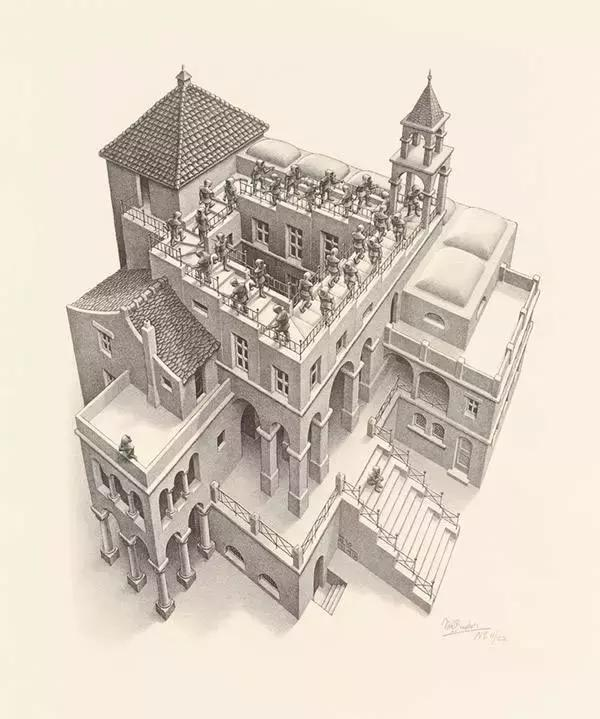
\includegraphics[width=1\linewidth]{./image/10-prop20-image12}

\hypertarget{ux7b2cux5341ux4e00ux8bfeux547dux9898ux4e8cux5341ux4e00}{%
\chapter{第十一课(命题二十一)}\label{ux7b2cux5341ux4e00ux8bfeux547dux9898ux4e8cux5341ux4e00}}

\hypertarget{ux547dux9898ux4e8cux5341ux4e00}{%
\section{命题二十一}\label{ux547dux9898ux4e8cux5341ux4e00}}

\textbf{如果在三角形的一边,从其端点,构建两条直线使相交于三角形内,这两条直线比三角形剩余的两边短,但夹角更大。}

学习欧几里得的证明题有不同的方式,最常见的有两种:一种是以阅读的方式顺着欧几里得的思路读下来,最好在阅读完毕之后能合上书自己再推演一遍;而另外一种方式则是只读命题,按照需求可以参考图片,然后想办法自己推演,看是否能有已知推出结论。

今天的命题二十一是一次高难度的挑战,一是我们尝试用英语上课,而是我们选择了第二种方法,希望能够推出欧几里得的证明。在自己亲自验证的过程中,希望Alex能明白,创造与跟随的区别以及创造时的助力(辅助线)。

如果我们阅读《几何原本》,总是感觉证明题并不难,逻辑非常的顺畅,然而只有我们在试图自行证明的时候,才发现逻辑的顺畅并不意味着线索的显而易见。我是指,信息就如同碎片一般,哪怕我们确定最后能组装成一个漂亮的拼贴画,拼贴画的轮廓和线条却不是那么容易就确定的。今天我和Alex一个小时的课就只在研究这一道证明题。

这道证明题的关键有两个:一个是辅助线,另一个是明确要引用的定理。

我们先来看题意:``如果在三角形的一边,从其端点,构建两条直线使相交于三角形内,这两条直线比三角形剩余的两边短,但夹角更大。''

这里需要比较两组不同的目标,一组是两条边之和,另一组是两个夹角。比较边和角分别要用到不同的定理,而前二十个命题比较边和夹角的定理并不多,尤其是上一个命题-命题二十-谈论的就是三角形两边之和大于第三边,很大可能性就会在此用到。之前命题关于角的大小则有对顶角、外角和三角形内角等比较,关于直角的命题可以暂时放在一边,因为一旦是直角,三角形就有了限制,而这道命题的陈述明显是针对一般三角形的。

将可以选择的命题放在一边,接下来就是辅助线的问题。我们一直都在强调选择辅助线的技巧,最核心的一点就是理解辅助线的作用。辅助线,顾名思义,是帮助完成命题的,而这个帮助就是一种桥梁的作用,换言之,辅助线就是一个媒介,帮我们从已知走向所求的证明。如果并不能很快的找到从已知到所求的桥梁,我们可以从不同的尝试开始,也就是我和Alex说,随便画,把你能想到的所有可能的辅助线都画出来,然后我们来对比分析它们在这个证明里的实用性。

Alex作图如下:(红色是辅助线)

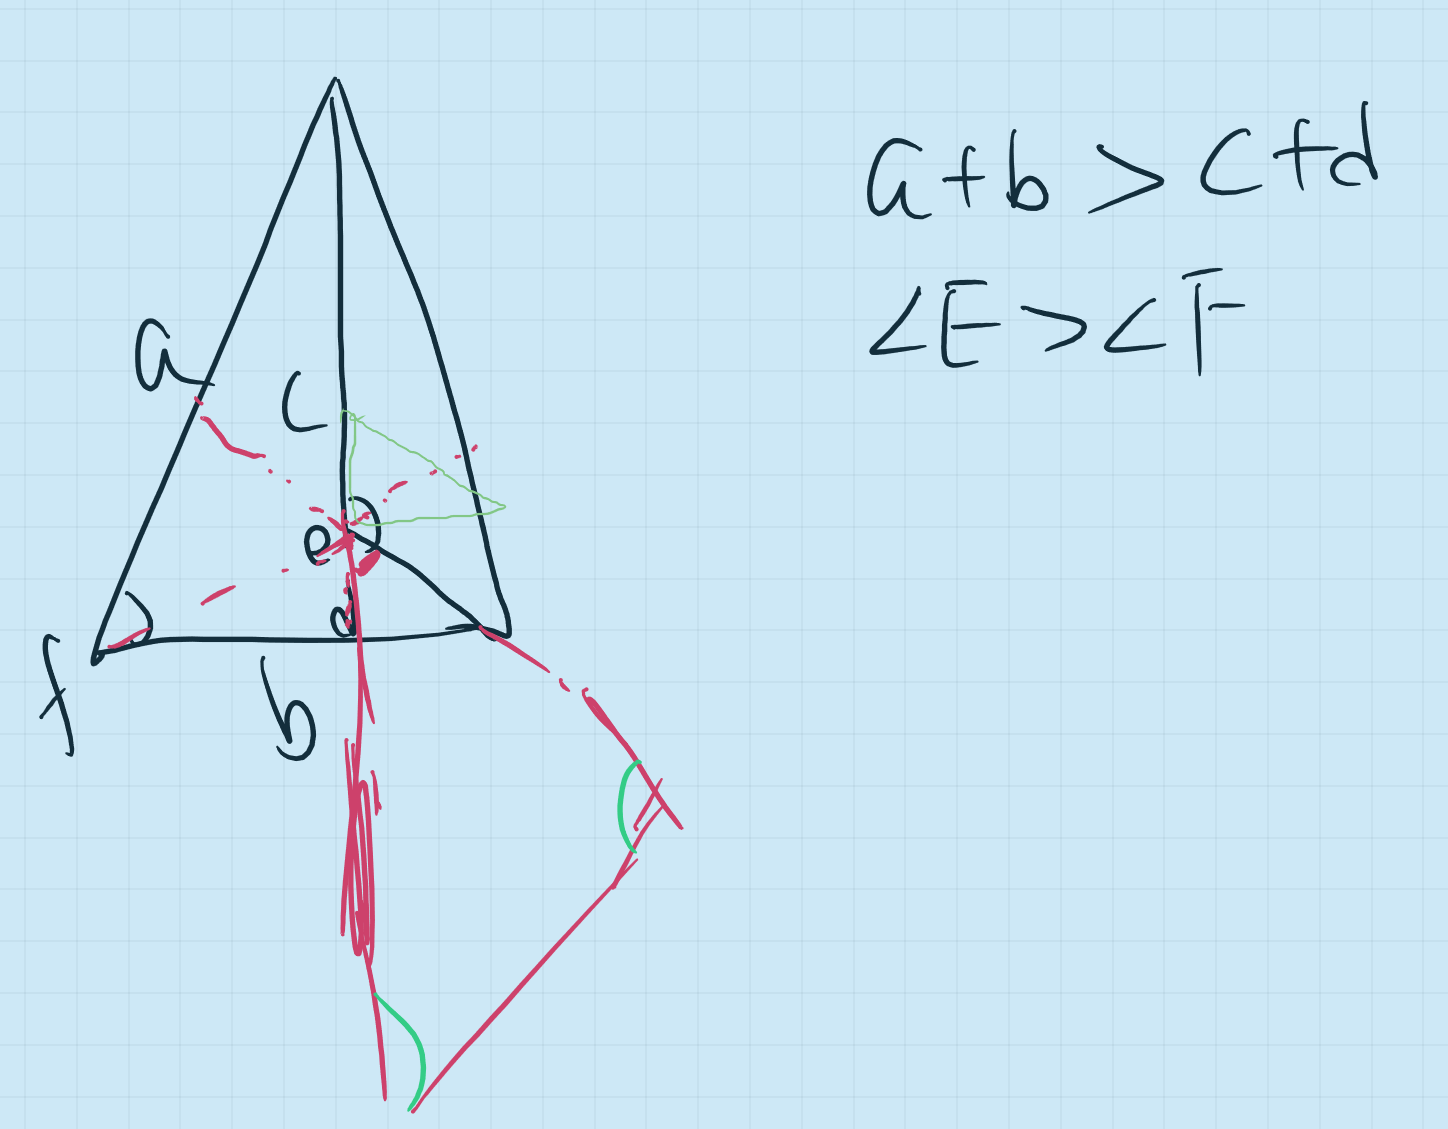
\includegraphics[width=1\linewidth]{./image/11-prop21-image10}

最后的辅助线起的一定是媒介作用,而媒介也就是过渡的意思,因为大多数的辅助线是尽可能的补充原有的图像,而不是进行重大的更新,换一句话说,辅助线往往是有限度的拓展。Alex的辅助线的思路在此就是跳跃太多,产生了很多新的线和角,都已经延伸到三角形之外了。其实红色的线已经包含了我们所期望的辅助线,然而也是因为太过细微,所以被忽略。学数学,思路开阔和细节到位两样都不可或缺。

这个时候就是需要追问:这条辅助线与什么命题/定理/性质联系在一起,可以被运用呢?如果没有答案的话,我们要排除掉这个辅助线,在这个过程中逐渐认识到辅助线``媒介''的特质。

当我们能够将辅助线和前面的命题相联系的时候,证明题的架构也就会变清晰了。这道题的辅助线是构建一个中间三角形,然后将角和边的对比从最里面的新三角形过渡到外面的三角形。相对于边的比较,角的比较相对简单,加了辅助线之后的角,对里面的小三角形是外角,而相对于外面的三角形则是外角,这种双重身份帮助实现了过渡的作用。边的比较看起来复杂,其实也是任意两边之和大于第三边与不等式加法相结合的运用,只不过中间的媒介在运用的时候绕了一个弯。

今天通过详细的学习命题二十一,希望Alex能够更好的理解辅助线的添加和运用。

参考作业:

\begin{itemize}
\tightlist
\item
  从最近的数学作业里挑5-10道用到辅助线的几何证明题,分析辅助线是怎么画的,然后辅助线是如何发挥过渡作用的。
\end{itemize}

\hypertarget{ux7b2cux5341ux4e8cux8bfeux547dux9898ux4e8cux5341ux4e8cux5230ux4e8cux5341ux56db}{%
\chapter{第十二课(命题二十二到二十四)}\label{ux7b2cux5341ux4e8cux8bfeux547dux9898ux4e8cux5341ux4e8cux5230ux4e8cux5341ux56db}}

九月开学之后,只能周末上课,那么每节课开始要花一点时间快速的回顾一下上一个命题。回顾命题二十一的重点也就是怎么添加辅助线,以及明确所用的定理。

命题二十二和命题二十算是一对证充要的组合,之前我们说的是任意三角形的任意两边之和都大于第三边,而接下来的命题二十二则是说任意三条线段,若其中两边之和大于第三边,则一定能构建一个三角形。也因此,命题二十是一道证明,而命题二十二是构建。

\hypertarget{ux547dux9898ux4e8cux5341ux4e8c}{%
\section{命题二十二}\label{ux547dux9898ux4e8cux5341ux4e8c}}

\textbf{由分别等于三条已知线段的线段构建一个三角形:那么必须满足任取其中两条线段,其和大于第三边。}

这道题首先是将给定的三条线段画到同一条直线上,然后取中间的边为底边,同时借助圆的半径相等的性质,将线段挪移到两圆相交的位置。这道证明题的关键也就是两圆相交所构建的新三角形的顶点。想象一下如果两圆不相交是什么样子?什么样的情况下两圆无法相交出顶点呢?无相交顶点也就是等价于无法构建一个封口的三角形。也就是两边之和小于第三边的情况。其实并不难理解,因为如果两边之和等于第三边,那么我们看到的是加粗的线段,互相重合;而如果两边之和小于第三边,就是开口的线条画,而无法围成图形了。如图所示:

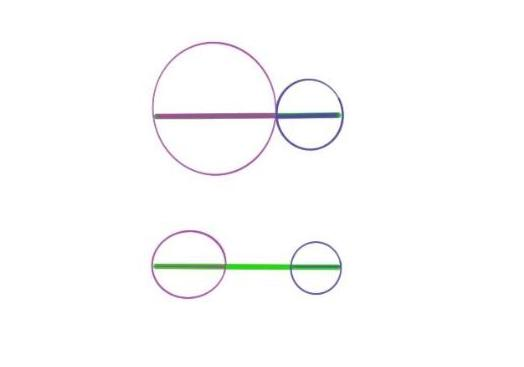
\includegraphics[width=1\linewidth]{./image/12-prop22-image11}

那么圆在这个构建的过程中起到了什么样的作用呢?它既是一个媒介,来传递等价的线段,同时又是一个检测手段,两圆的关系,相交,相切,还是不相交也不相切,它等价于三边的关系也决定了三角形的构建。

\hypertarget{ux547dux9898ux4e8cux5341ux4e09}{%
\section{命题二十三}\label{ux547dux9898ux4e8cux5341ux4e09}}

\textbf{从给定的直线上一点,构建一个直线角,使等于给定的直线角。}

命题二十三并不难,这里最值得讨论的是角和三角形的关系。首先先让Alex来发散思维,说一下他所能想到的角和三角形关系的论述。Alex说的第一条是三角形内角和一百八十度,第二条是外角比其它两个内角要大。这开头两条都是三角形的性质,而我们希望触及的问题是角是什么?它能独立于三角形存在么?而思考这样的问题是因为,在证明中,欧几里得选择用构建三角形再证其中某角相等的方式。为什么要这样做呢?

这里角的定义参考定义八和定义九:

\begin{quote}
定义八:平面角是,在同一个平面内,其中一条线与另一条线相交但不重合的倾斜度。
\end{quote}

\begin{quote}
定义九:当包含角的线是直的时候,这个角被称为直线角。
\end{quote}

很明显,在最开始定义角的时候,是不需要将其放在某在直线围成的图形中的,比如三角形。那么三角形在这里的作用是什么呢?

三角形这里相当于一个媒介,以允许我们应用之前学过的三角形的性质来对其中含有的角进行比较。如果我们直接将角进行比较的话,也可以用位移和重合来进行论述,但显然欧几里得是试图避免这样的证明的。如果不直接对比,还可以将角进行切分等方式,部分部分的进行比较。而这里选择三角形,则是一种填充的方式,将小的部分放入大的整体中,以方便鉴别。这几种可能性代表了不同的思考方式:

\begin{itemize}
\tightlist
\item
  直接比较法: 即将所需要比较的对象进行直观的整体性比较
\item
  细节对比法:将所需要比较的对象的细节按照需要进行划分,并一一对比
\item
  填充对比法:将所需要比较的对象放到更大的文本/环境中,通过与整体或其它部分的相配合进行选择。
\end{itemize}

对应到现实生活中,在学校系统里就是直观的总分比较;单科成绩比较;看排名;如果是应聘的话,就是整体印象;简历细节;团队合作表现。

\hypertarget{ux547dux9898ux4e8cux5341ux56db}{%
\section{命题二十四}\label{ux547dux9898ux4e8cux5341ux56db}}

\textbf{如果两个三角形的两边分别对应相等,但是它们的夹角,其中一个比另一个大,那么相应的底边也长于另一个底边。}

关于命题二十四,我们没有讨论太多,命题二十四和命题二十一遥相呼应。命题二十一是固定住底边之后,看其它两边和顶角的大小状况;而命题二十四则是固定住两边长度之后,看底边与顶角的变化。
这道题在证明上的关键是将所要比较的两条边放入同一个三角形之中,然后通过所对角大小的对比来证明两条边的长短关系。

参考作业:

\begin{itemize}
\tightlist
\item
  任意选取一个录取/竞赛系统,分析该系统下的比较框架。
\item
  指定一个购买物品类型(譬如扫地机器人),分析当下市场上的现有产品,选择你会购买的产品并陈述理由
\end{itemize}

\hypertarget{ux7b2cux5341ux4e09ux8bfeux547dux9898ux4e8cux5341ux4e94ux5230ux4e8cux5341ux516b}{%
\chapter{第十三课(命题二十五到二十八)}\label{ux7b2cux5341ux4e09ux8bfeux547dux9898ux4e8cux5341ux4e94ux5230ux4e8cux5341ux516b}}

接上节课末尾的二十四,先复习一下,并看命题二十五。

\hypertarget{ux547dux9898ux4e8cux5341ux4e94}{%
\section{命题二十五}\label{ux547dux9898ux4e8cux5341ux4e94}}

\textbf{如果两个三角形的两边各自对应相等,但是其中一个底边更长,那么它们的夹角更大。}

命题二十四和命题二十五是连接在一起的,甚至非常相像,都是在固定好三角形的两条边之后,看顶角和底边的关系。命题二十四是说大的顶角对应长的底边,命题二十五则是反过来又证了一遍,长的底边对应大的顶角。如果我们将命题二十四和命题二十五放在一起看,会发现,两个都是归谬法,并且他们反证的方法都是首先排除掉了相等,再排除掉小于的情况。这这里我再一次询问了Alex对反证法的感觉,是否觉得其有足够的说明力,Alex这里用了一个比喻:归谬法好像是二进制,似乎只考虑0和1,那如果还有其它隐藏的情况呢?这个问题很好地揭示了归谬法的局限性,反证,就是证明声明以外的情况是错误的,因此只能承认声明的正确性。

其实这里最薄弱的环节并不是证明其它情况的错误性,而是在枚举所有情况的时候并没有列出所有的可能性。在欧几里得的证明里,是考虑三种情况,大于,等于,和小于。假设我设一个抽象世界是现实生活的翻版,没有完全相同的存在,``不等系统'',那么我在这个新的系统里证明的时候是不是就永远可以不考虑等于的情况?站在欧几里得的系统里,是不是因为相等的可能性存在就能推翻很多``不等系统''里的命题?那么存不存在另一个新的系统与欧几里得系统的关系就如同欧几里得系统与``不等系统''的关系,在另外一个角度可以发现除了大于,小于和等于之外的情况,比如说``约等于''?那么这个时候,归谬法所证明的命题是不是就都失效了呢?而这个``约等于''的存在却不影响其它的证明?那么我们是不是能声明归谬法的论证不够有说服力?

关于命题二十四和命题二十五还有一个值得思考的地方。为什么要证二十四在二十五之前?这里的顺序是否能颠倒呢?如果看证明里的援引,会发现命题二十四需要引用命题二十三,二十三会用到二十二,似乎先二十四后二十五这个顺序是从二十二开始就在准备了,如果我们希望先证长边对大角(二十五),再证明大角对长边(二十四),你能做到么?是否需要额外的命题辅助呢?课下不妨仔细思考一下。

\hypertarget{ux547dux9898ux4e8cux5341ux516d}{%
\section{命题二十六}\label{ux547dux9898ux4e8cux5341ux516d}}

\textbf{如果两个三角形中的两角各自对应相等,并且其中一边等于另一边,即或者等角的临边,或者等角的对边,那么它们剩余的边和角也都对应相等。}

命题二十六很长,Alex说看到就觉得``长,烦,难'',但其实长的命题未必难,有时候有的短命题是另辟蹊径来证明的,反而更难思考,命题二十六只是长,如果我们将它分模块处理,就会变的简洁了。命题二十六主体分为两部分,第一部分是ASA,第二部分是AAS,每个部分分别又都证明在ASA与AAS的情况下,三角形剩余的部分都相等。而且它证明的格式都是一样的,假设剩余的某一组对应的边并不相等,设其中一个边长于另一个,但是这会导致对应的角出现不可能的情况,因此余边必须相等,那么余角也要相等。这样将命题二十六先拆成两半,每部分就都和之前的命题一样不算长了,然后仔细看其中一半,剩余的一半也就很快看懂。

这个命题对之前证明全等的方法进行补充,到此,SSS,SAS, ASA, AAS四种证明全等的方法就都证完了。
在实际的上课过程中,其实是和Alex先一起学习了命题二十七和命题二十八,因为正好学校的数学课也在讲平行,我们不仅一起看了欧几里得的证法,同时看了教材上选读的证明。对比两个证明,我们一致投票给欧几里得。这里之所以可以将学习证明题的顺序进行调换,是因为命题二十七上接的最远的命题是命题十六,从命题十七到命题二十五,和命题二十七并不直接相关。我们可以这么理解,尽管命题后的数字是顺序递增的,而事实上从命题十六之后发展出互不打扰的两个分支,一个是十七到二十五,另一个方向是从二十七开始,这两个方向在之后会交叉。此时我只是希望Alex注意到这一点,在第一卷结束,我会希望Alex能够手绘或者用思维导图做一份命题之间的连接图,从一个更宏观的视角看第一卷四十九个命题的逻辑线。

\hypertarget{ux547dux9898ux4e8cux5341ux4e03}{%
\section{命题二十七}\label{ux547dux9898ux4e8cux5341ux4e03}}

\textbf{如果一条直线落在两条直线上并使得内错角互等,那么两条直线平行。}

命题二十七和命题二十八都是与平行相关的,且都是关于判断平行的条件,之后我们会学习平行的性质(命题二十九)。这里我们再次回顾一下平行线的定义:

\begin{quote}
定义二十三:平行直线是在同一个平面,向两个方向无限延伸并互不相交的直线。
\end{quote}

只看定义二十三,我们也能明白这个定义是无法帮助我们判定一组平行线的,因为它要求在无限远的地方直线仍不相交,而我们的证明题在具象化的时候都是证明在当下,也因此我们需要重新设定其它判定条件,等价于无限延伸且不相交,或者是由于这个无限延伸而不相交进一步推导出来,可以放置于和平行中间的地带,命题二十七就是这样诞生的。内错角互等的情况下,直线两个方向延伸而都不相交,也就满足定义平行了。

\hypertarget{ux547dux9898ux4e8cux5341ux516b}{%
\section{命题二十八}\label{ux547dux9898ux4e8cux5341ux516b}}

\textbf{如果一条直线落在两条直线上并使得同位角相等,或者同旁内角之和等于两直角,那么两条直线平行。}

命题二十八其实可以拆分成两个小命题:

\begin{itemize}
\tightlist
\item
  同位角相等,两直线平行;
\item
  同旁内角互补,两直线平行
\end{itemize}

这个证法并没有通过定义直接证明平行,而是转换为命题二十七来证平行,使得步骤更加简练。

参考作业:

\begin{itemize}
\tightlist
\item
  在你喜欢的策略类游戏里,找到那些不会立刻起作用但是要提前完成的的游戏操作,并且解释原因。
\end{itemize}

\hypertarget{ux7b2cux5341ux56dbux8bfeux547dux9898ux4e8cux5341ux4e5dux5230ux4e09ux5341ux4e8c}{%
\chapter{第十四课(命题二十九到三十二)}\label{ux7b2cux5341ux56dbux8bfeux547dux9898ux4e8cux5341ux4e5dux5230ux4e09ux5341ux4e8c}}

上节课学习了平行线的判定条件,命题二十九接下来讲了平行线的性质,并且将三个性质整合在了一个命题当中,且这三个性质其实就是命题二十七和二十八中的判定条件。命题二十七,二十八与命题二十九构成了我们之前上课所学习到的一组充分必要条件。

\hypertarget{ux547dux9898ux4e8cux5341ux4e5d}{%
\section{命题二十九}\label{ux547dux9898ux4e8cux5341ux4e5d}}

\textbf{落在两平行直线上的直线,会使得内错角互等,同位角互等,同旁内角之和等于两直角。}

命题二十九在证法上,则是填充对比法,我们需要用添加角再次组合的方式来证相等。

\hypertarget{ux547dux9898ux4e09ux5341}{%
\section{命题三十}\label{ux547dux9898ux4e09ux5341}}

\textbf{与同一直线平行的直线们,也互相平行。}

命题三十是利用平行的性质进行了进一步的推论。这里我们回忆起公理一:与同一事物相等的事物们彼此互等。这个公理的行文方式与命题三十的声明如出一辙:``与同一直线平行的直线们,也互相平行。`` 这对我们有什么启发呢?这个证明的信服力是否能超越公理一?(为什么感觉似乎并不如此呢?)
让我们想象直线A与B各自延伸永不相交,但是直线A投影在直线B上的直线C与A平行,与C相交。然而不要被这个想法迷惑,因为回到平行的定义,(平行直线是在同一个平面,向两个方向无限延伸并互不相交的直线。)是需要直线在同一个平面上的。尽管命题三十没有写出同一个平面的隐含条件,然而它还是存在的,也因此这个想象被排除在了欧几里得的世界之外。是不是总是想要找到欧几里得的破绽却最后还是钦佩这个系统的严谨性?

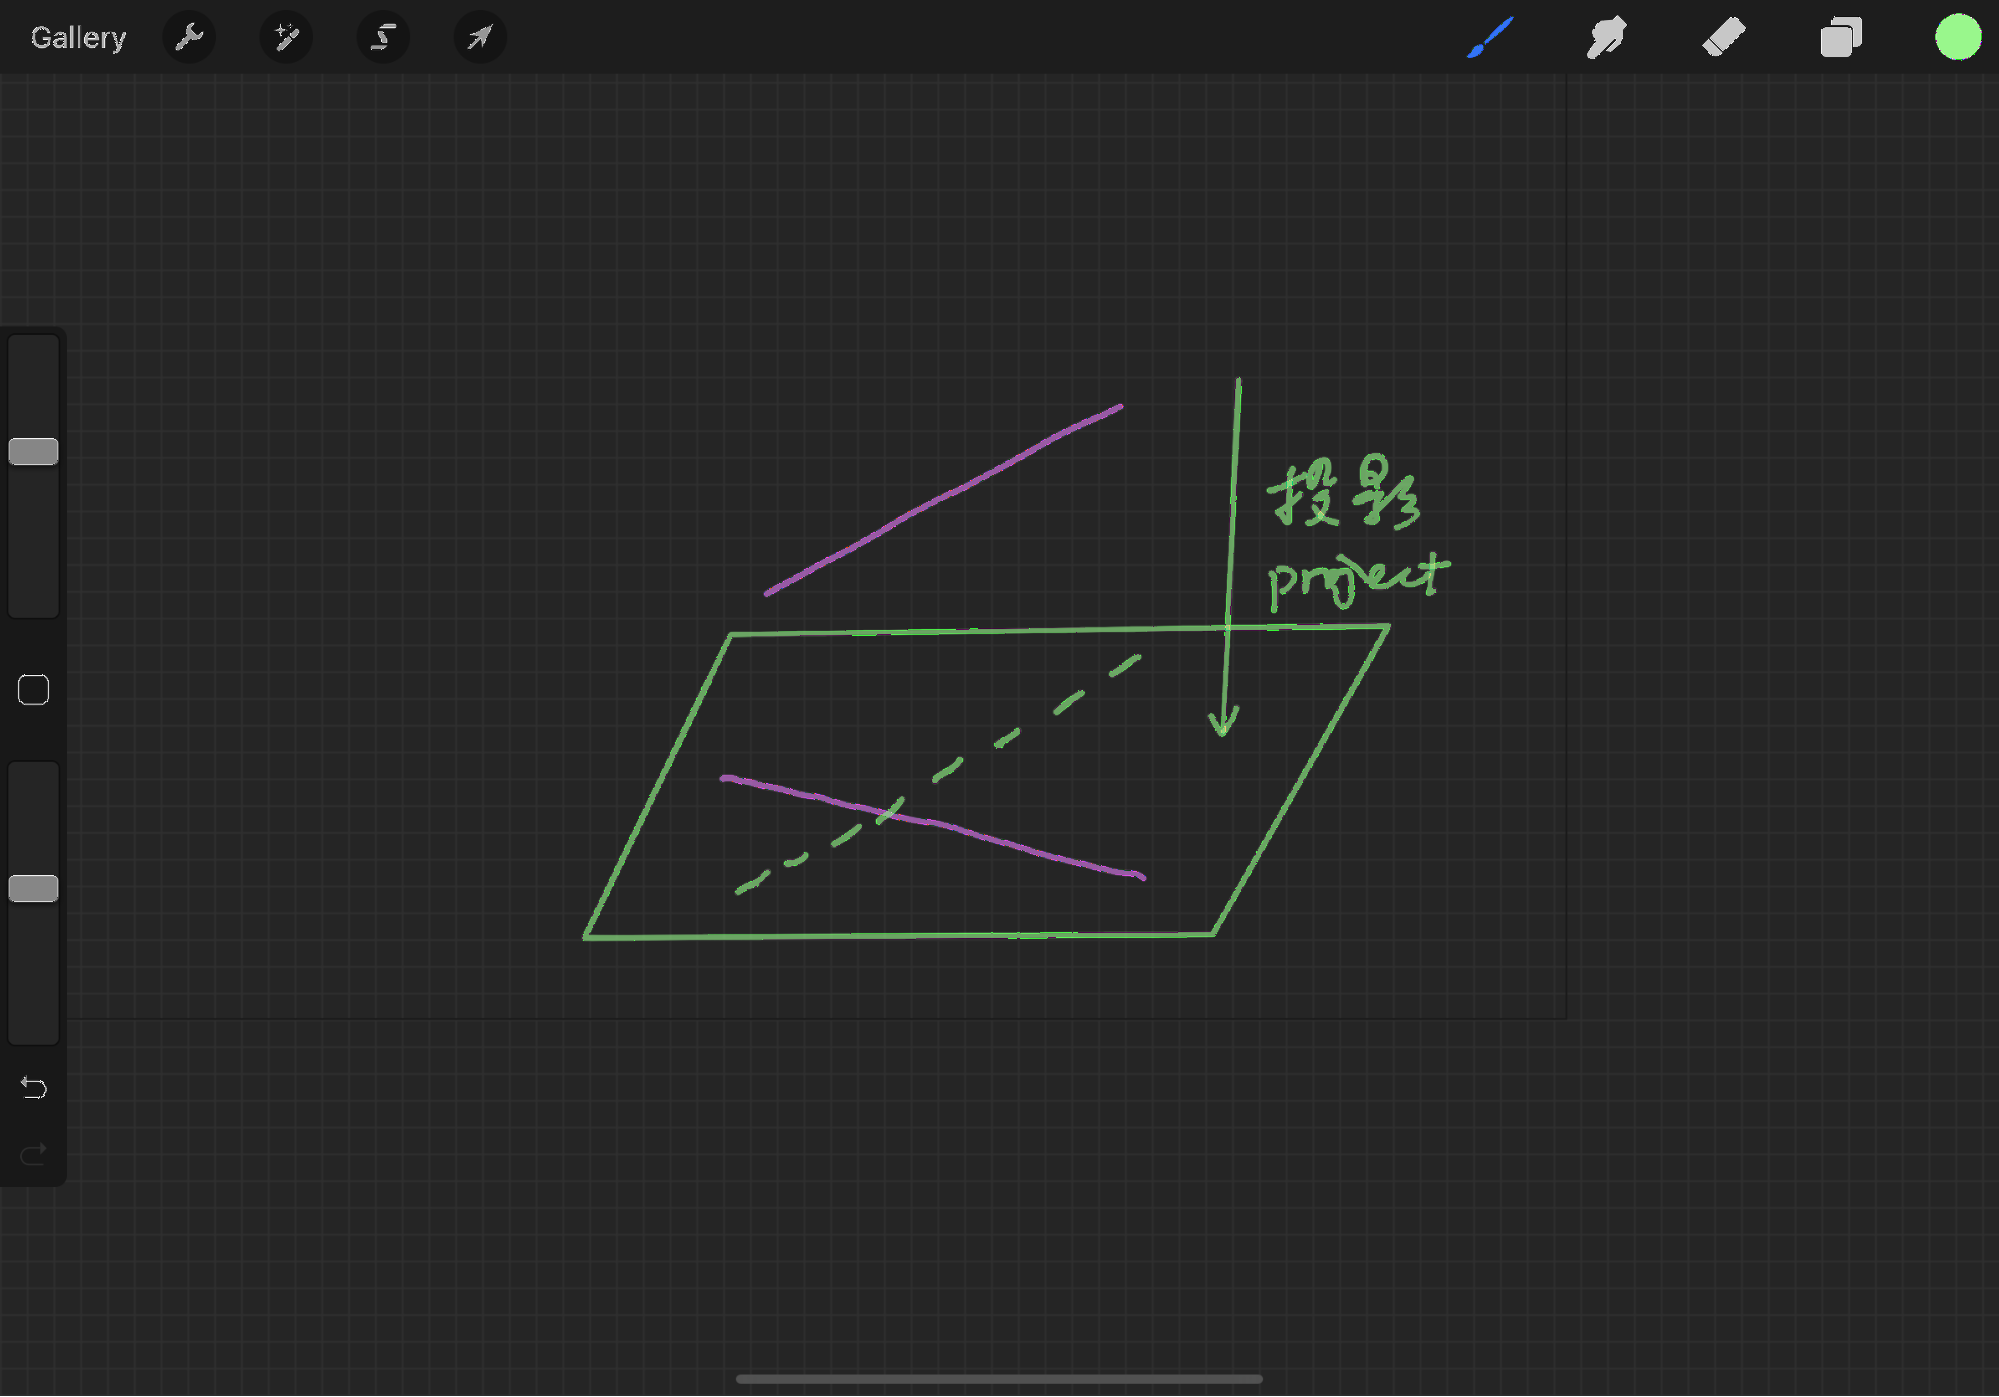
\includegraphics[width=1\linewidth]{./image/14-prop30-image13}

\hypertarget{ux547dux9898ux4e09ux5341ux4e00}{%
\section{命题三十一}\label{ux547dux9898ux4e09ux5341ux4e00}}

\textbf{过定点,画一条直线,使平行于另一条直线。}

命题三十一的证明过程十分轻松愉快,而这里值得讨论的问题是,是否过一个定点对一条直线,只能画出一条平行线?这里的唯一性意味着什么呢?在学习平行定义的时候,我们曾经讨论,是否可以用''两条直线上各对应点之间的距离永远相等``来取代''两个方向延伸但并不相交``这个说法,看到命题三十一中所隐含的唯一性这个特点,能否感觉到''两条直线上各对应点之间的距离永远相等``这个特性?那么为什么欧几里得没有用这个方式去进行定义呢?在我眼中,这个问题绕了一圈又回到了定义四:直线是线,这条线均匀地铺于其(线)上的点。

欧几里得并没有完全定义线和点之间的关系,我们并不能够将无限相连点之间的的相等距离等价到两条直线之间的距离等价。这个点到线的巨大鸿沟才是定义平行线时的困难。

另外,命题十二(给定一无限直线,在线外一给定点上,画垂线。) 垂线似乎也是唯一的,并且垂线是通过证明两个相邻角互等而作出的。平行线则是通过证明内错角相等而证出的。在命题二十二的时候我们有看到从线到角到图形的脉络,而画垂线和画平行线这里的证明则意味着,从角到线的回路也是相通的。

\hypertarget{ux547dux9898ux4e09ux5341ux4e8c}{%
\section{命题三十二}\label{ux547dux9898ux4e09ux5341ux4e8c}}

\textbf{在任意三角形中,如果延长一边,那么外角等于两内对角之和,且三个内角的和等于两直角。}

命题三十二是两个部分,总体来讲,承接了命题十六(在任意三角形中,如果延长其中一边,那么外角大于(任一)内对角。)和命题十七(在任意三角形中,以任意方式取任意两角,其两角(之和)小于两直角)。我们会发现当我们证明完命题三十二的时候,十六和十七就基本不会再被调用了,因为它默认包含在了命题三十二的涉及内容之中:外角等于两内对角之和,自然也就大于任一内对角,三个内角的和等于两直角,那么三个角中其中任意两个之和也就必然小于两内角。

尽管看起来命题十六十七到命题三十二也不过是往前进了小小的一步,然而这个过程却是艰辛无比,不能省略的。就好像你在一把伞从骨架到加上伞面,似乎只是盖上了伞面,然而伞面需要多步骤的工艺来实现它,然后才能装到伞架上。

另外关于命题三十二,Alex自己想了一个不同的证明方法,也是非常可行的。

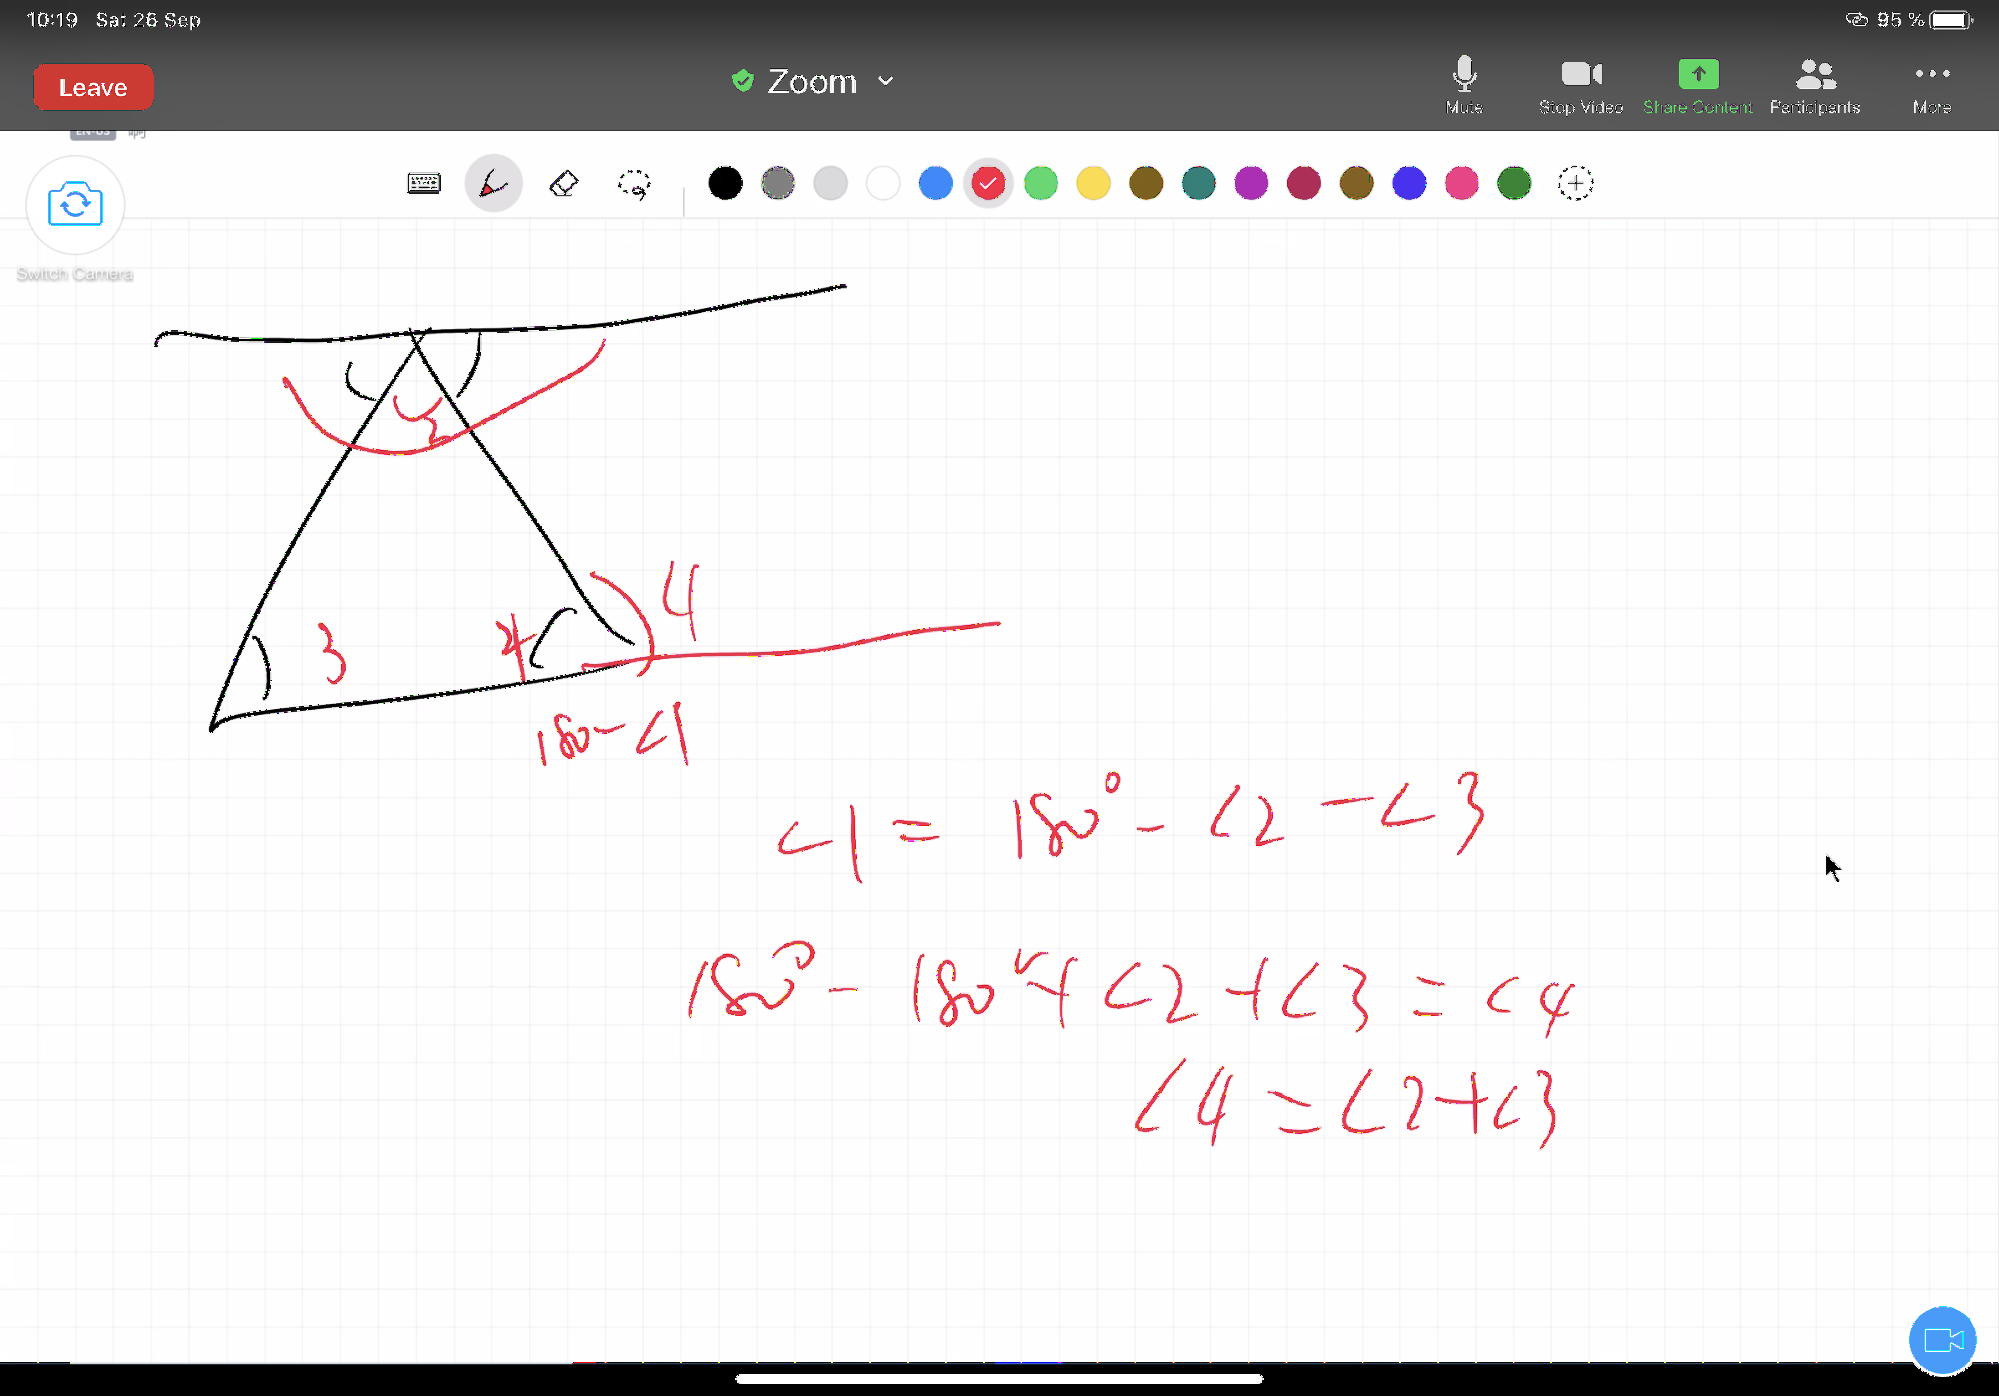
\includegraphics[width=1\linewidth]{./image/14-prop32-image14}

\hypertarget{ux7b2cux5341ux4e94ux8bfeux547dux9898ux4e09ux5341ux4e09ux5230ux4e09ux5341ux516d}{%
\chapter{第十五课(命题三十三到三十六)}\label{ux7b2cux5341ux4e94ux8bfeux547dux9898ux4e09ux5341ux4e09ux5230ux4e09ux5341ux516d}}

这一节课的命题是关于平行四边形的。我们把今天要研讨的命题分为两组,命题三十三和三十四一组,关于平行四边形的定义和性质;命题三十五和三十六一组,关于面积相等概念的转移。

\hypertarget{ux547dux9898ux4e09ux5341ux4e09-ux4e09ux5341ux56db}{%
\section{命题三十三 \& 三十四}\label{ux547dux9898ux4e09ux5341ux4e09-ux4e09ux5341ux56db}}

\textbf{命题三十三:向同一方向「分别」连接相等且平行线段「端点」的线段也相等且平行。}

\textbf{命题三十四:在平行四边形的区域内,对边及对角互等,且对角线平分该区域。}

在命题探讨完三角形,平行之后才轮到平行四边形,然而有意思的是,如果我们回头看定义的顺序,平行四边形其实在定义二十二就已经存在了,但是是在平行直线之前出现的,并没有以平行四边形的名字出现,在定义中也没有用到平行这个概念------对边对角相等但四边不全相等且不为直角的是斜方形?(节选定义二十二),这里我们不妨停下来想一下,对边对角相等的四边形,两组对边是不是一定平行?那么我们之前为什么不通过平行四边形来证平行线?而是通过了内错角、同位角和同旁内角的关系?这里回顾命题二十三:从给定的直线上一点,构建一个直线角,使等于给定的直线角。在这个证明里面欧几里得就是把角放在三角形里面,通过证明三角形全等来证两直线角相等的。

大概三角形和平行四边形有一个不同的地方。平行四边形是两组平行线,并且一组平行线是可以独立存在的,当两组平行线在特定的情况下产生交叉,才会出现一个平行四边形。两组平行线互相依赖产生新的图形,而平行这个概念却是可以从四边形中独立出来的。三角形是可以视为一条直线折两折之后的图形,与它相关的延长线,外角等都依赖于三角形存在,它本身已拆无可拆。因为三角形可以作为一个基本单位,而平行四边形不可以。

于是在命题的学习中,我们先了解平行的概念,然后在一组平行线上搭建另一组平行线,就构建了一个平行四边形,然后证明它的性质满足于``对边对角相等但四边不全相等且不为直角''这个定义的部分,之后两者的概念才产生重合,也完成了从已知到被证明的角色转换。命题三十三就是在平行的基础上搭建平行四边形,而命题三十四证明了平行四边形的对边对角互等。很有意思的是,命题三十三的行文中并没有提到``平行四边形'',而只是说另一组对边平行且相等,而命题三十四就紧接着以平行四边形的区域开篇了。

在命题三十四中,出现了''area``,并没有被定义,而在之后会演变为面积,现在姑且让我们用``区域''来描述它,也就是被线圈定的地方。之前我们谈论过角的平分,线的平分,却是第一次谈论图形的平分。在命题九中,我们曾用两个全等三角形,来确认平面角是被平分了,也就是我们先确认了两个图形的相等性,然后又取出了其中角的部分。而这里,我们第一次直接的谈论图形(区域)。

这里可以引发无数的想象和思考,这个图形是什么样子的?是虚幻还是实体,是被线条如同栅栏般圈起来的封闭内容么?还是与线条紧密相连不可分割的存在?它本身可以和图形分离出来么?在生活中似乎两者例子都能找到的,比如说院子,那么线条就是围墙,而计算院子内的面积,是和墙本身分离的,因为希望知道院子的土地面积,可以种多少花花草草。而如果买一个生日蛋糕,就又是另一码事了,蛋糕的边缘和蛋糕本身是一个整体,图形和边是连续在一起的,我们对院子和蛋糕分别进行抽象化处理,都是几何图形,而边和内里区域的关系却大不相同,这能带给我们什么样的思考呢?

\hypertarget{ux547dux9898ux4e09ux5341ux4e94-ux4e09ux5341ux516d}{%
\section{命题三十五 \& 三十六}\label{ux547dux9898ux4e09ux5341ux4e94-ux4e09ux5341ux516d}}

\textbf{命题三十五:同底且在同组平行线之间的平行四边形互等。}

\textbf{命题三十六:等底且在同组平行线之间的平行四边形互等。}

以上两个命题的证明方法并不难,命题三十五的证法是对等量减去等量又添加等量的方法,而命题三十六在之前命题的基础上,只需要找到合适的媒介作为中间桥梁就可以了。

有意思的是相等概念的扩充。相等这个比较的行为是从来没有被定义过的,它似乎是从现实生活中的概念直接拿过来用的,之前我们所证明的事物大多是因为重合而相等,也就是说希望被证明相等的部分可以作为一个连续的整体,每一个不可切割的部分都能一一对应。因为重合的物体是可以分开的,那么经过运动,先重合又不重合的两个物体就是相等的,这里的分离运动有一个假设的前提,就是它的分离必须是无任何损耗的。比如说平移,翻转,对称这些运动,我们假设在抽象几何世界中,不会产生任何能量的损耗,这才会有运动分离之后的相等性。(对于一个位移的物体,也有这样的运动前提,我们假设了这个物体在位移中没有损耗,否则运动前的它和运动后的它就不一样了)

相等的第一步,是从重合到局部分离,也就是命题三十五的同底,然后则是完整的分离,命题三十六中已经变为了等底,同时,在两个命题中,都隐含着脱离形状桎梏的情况,同底但角并不同,在同组平行线之间的同底平行四边形,形状并不一样,而在命题三十五中也被证明了他们的相等性,是以拼接的方式完成的,也就是说我们可以将两个平行四边形进行切割组合,他们所分成的部分,在形状上是一致的,由此推出整体的相等性。这就是改变视角,回到局部和微观部分进行证明的例子。如果我们认可了这样的逻辑跳跃,那么几何会突破我们的视野限制,带我们进行到接近无限的情况。想象一个接近与一根直线的平行四边形,它的底固定,而斜边接近无限长,虽然不知道到底有多长,但是它的面积却是已知的,因为可以通过同底同组平行线之间的其它平行四边形得知,这一个从无限到有限的跳跃,很是值得玩味。

\hypertarget{ux7b2cux5341ux516dux8bfeux547dux9898ux4e09ux5341ux4e03ux5230ux56dbux5341ux4e8c}{%
\chapter{第十六课(命题三十七到四十二)}\label{ux7b2cux5341ux516dux8bfeux547dux9898ux4e09ux5341ux4e03ux5230ux56dbux5341ux4e8c}}

命题三十七和三十八是对命题三十五和三十六的一个再加工,紧接着,我们将条件翻转,在命题三十九和命题四十以图形来倒推平行线。四十一是一个拓展,而四十二是在这一系列基础上的一个再创造。这些命题本身都很短,在掌握命题三十五和三十六的基础上,证明过程也相对简单。

\hypertarget{ux547dux9898ux4e09ux5341ux4e03}{%
\section{命题三十七}\label{ux547dux9898ux4e09ux5341ux4e03}}

\textbf{同底且在同组平行线之间的三角形互等。}

命题三十七是命题三十六的一个延续,在证明平行四边形是等量的基础上,证明等量的一半也相等即可。在命题二十三的时候我们提到过不同的证明思路,此处是运用了以大推小的填充对比法。之前我们为了对比角的大小,倒回三角形的层级来进行比较,而现在我们为了证明三角形的大小,更进一步推到了平行四边形的比较上。然而有趣的是,如果我们用宏观的视角来看第一卷,它基本上是遵循从角到图形顺序,然后每一次的跳跃又都可以倒回一小步对之前局部的性质进一步说明。其实这也给我们一个生活和学习上的启示,有些成果是在一个部分进行细加工得来的,而有些成果的发现则需要跨越视角后在看,在同一个知识点不需要过去求善求美,学到更深的内容的时候会理解的更好。

另外命题三十七里比较争议的其实就是最后一步,我们是否可以理所当然的使用``等量的一半也相等''这个论证。因为在公理对等量的运算中,是不涉及乘法和除法的,只是说了加减相等的量也相等。我们可以将论证内容改写为,等量减去一半量后也相等,这是就是运用了公理三,但是怎么才能如何将量取一半呢?这里也就是命题三十四提到的对角线平分平行四边形的部分了。注意这里对公理三的改写运用是有争议的,但是此处合理,是因为平分平行四边形在命题三十四那里得到了证明。

\hypertarget{ux547dux9898ux4e09ux5341ux516b}{%
\section{命题三十八}\label{ux547dux9898ux4e09ux5341ux516b}}

\textbf{等底且在同组平行线之间的三角形互等。}

命题三十七和三十八的顺序是完全复制了命题三十五和命题三十六。与命题三十七相同,命题三十八只是在证明同样条件下平行四边形相等的基础上加了最后一句相等的量的一半也相等,就结束了证明,同样的方法和争论不再赘述。

\hypertarget{ux547dux9898ux4e09ux5341ux4e5d}{%
\section{命题三十九}\label{ux547dux9898ux4e09ux5341ux4e5d}}

\textbf{同底的同侧全等三角形在同组平行线之间。}

之前的命题是是通过平行线和底边的关系来证明三角形之间的联系,现在则是限定三角形来看平行线。让我们来思考一下,平行线意味着什么?首先,如果我们只是有两个同侧同底的三角形,这个共同的底边就是其中一条平行线的一部分,然后另一条平行线在最开始是不显示出来的(注意,这里不能说不存在,因为它一直存在,只是我们有没有发现它且将它标出来),是需要我们连接两个三角形的顶点才能绘制出这条平行线的一部分。那么画出的这条平行线其实是在一定程度上圈定了三角形的领域范围,也就是上下的边界,而这个被找到的边界之间有着平行的关系。这能给我们什么启发呢?假设我们在观察一个事物,那么也要去思考一下那些不是偶然的相关联的更大范围事物的性质。由之前的命题得知,这里将两三角形的顶点连线出现的性质并不是一个偶然,这种必然就是新命题值得明确化的方向和内容。

\hypertarget{ux547dux9898ux56dbux5341}{%
\section{命题四十}\label{ux547dux9898ux56dbux5341}}

\textbf{等底的同侧全等三角形在同组平行线之间。}

命题四十的来源存疑,被记载是编者后期补充的,然而它承接命题三十九,同时它从``同底''到``等底''的平行变换符合欧几里得之前证明题的作风, 我个人认为,哪怕它是编者补充的,保留下来也无可厚非。

\hypertarget{ux547dux9898ux56dbux5341ux4e00}{%
\section{命题四十一}\label{ux547dux9898ux56dbux5341ux4e00}}

\textbf{如果一个平行四边形和一个三角形共底且在同组平行线之间,那么此平行四边形是三角形的两倍。}

在将平行四边形和三角形在底边相等且同组平行线之间的情况分别证完以后,(额外又增添了反证平行线内容),终于我们看到了将平行四边形和三角形整合在一起的证明。命题四十一就是限定了同底和平行线的条件,将命题三十五和三十七进行了一个推论。此处值得注意的的是两倍的这个概念,不要忘记我们的一个历史遗留问题,命题三十四中关于``area''的讨论,此处的图形面积是否可以进行比较,比较的基准线是什么?尽管书中从来没有提到面积单位的问题,但是在我们进行比较的时候,面积单位是不是已经被假定存在了呢?这一点一直都没有被重视,这个单位的问题我们在第五卷的定义还会进行更进一步的探讨。

\hypertarget{ux547dux9898ux56dbux5341ux4e8c}{%
\section{命题四十二}\label{ux547dux9898ux56dbux5341ux4e8c}}

\textbf{用一个给定的直线角构建一个平行四边形,使之等于给定的三角形。}

整本书的开头是在一条直线上构建一个等边三角形。这也不禁让我们思考,数学的意义是在于发现还是创造,或者说再利用?这也是我曾经让Alex想过的一个问题。之后我们还在此构建三角形(命题二十二),直线角(命题二十三),画了平行线等。此处是构建平行四边形,但给了两个限定条件,一是限定角的大小,二是限定面积的大小。因为前一道命题已经证明了同底的平行四边形和三角形两倍的面积关系,那么自然而然,同组平行线内,底边一半的平行四边形面积和三角形相等,所以只需要在画平行四边形的时候使得角的大小与给定角相等即可。从命题三十五到这个命题,都是关于同组平行线之间四边形和三角形的来回转化,也是对一类平移转换技巧的反复使用,从重合到局部分离到完全分开,再到整体和部分之间的比较,以及停在重塑,也就是在创造上。数学的目的不仅仅是帮助我们认知自然规律,从一开始就有着再创造的含义。

\hypertarget{ux7b2cux5341ux4e03ux8bfeux547dux9898ux56dbux5341ux4e09ux5230ux56dbux5341ux4e94}{%
\chapter{第十七课(命题四十三到四十五)}\label{ux7b2cux5341ux4e03ux8bfeux547dux9898ux56dbux5341ux4e09ux5230ux56dbux5341ux4e94}}

\hypertarget{ux547dux9898ux56dbux5341ux4e09}{%
\section{命题四十三}\label{ux547dux9898ux56dbux5341ux4e09}}

\textbf{在任意一个平行四边形中,关于对角线的补形互等。}

这道题用一句话概括就是反复套用公理三,等量减等量再减等量的余量始终相等。一组全等三角形减去两组小全等三角形,剩余的四边形面积仍相等。证明题不难,记住新的概念补形指代的区域即可。另外就是这道题很形象的诠释了面积和形状分离的概念。两个补形面积相等但形状不同,隐含着数学中相等的概念侧重于面积(质)而非形状(形),数学想要思考和比较的内容是超越视觉意识的。

\hypertarget{ux547dux9898ux56dbux5341ux56db}{%
\section{命题四十四}\label{ux547dux9898ux56dbux5341ux56db}}

\textbf{用给定的线段和直线角作平行四边形,使等于给定的三角形。}

命题四十四是前面命题四十二的升级版,命题四十二在限定与已知三角形同底的情况下,限定角的大小和面积画平行四边形,这里命题四十四,将底边的位置再一次进行了一个挪动,也就是与三角形更彻底的分离开来,只保留面积上的关系,而彻底没有了位置上的联系。结合之前的命题来看,可以发现欧几里得的证明都是最终走向独立性的,发现联系,同时又让它们分离能独自存在而不受干扰。那么为什么这道命题没有在证完四十二之后紧接着证明呢?此处复习一下之前讲过的内容。因为命题四十三也是推理的一部分,而命题四十三被单独出来,也说明它有自己独立存在的价值,可能在后面会被其他证明反复引用。如果我们将第一卷整卷内容放在一起,抽调所有的命题声明,那么本身也是一个大的论述,然而我们将它又切割成不同的部分,进行声明,是为了更好的对某一个部分的反复使用,便于定位和查找。(编程写代码也是同样的道理)

\hypertarget{ux547dux9898ux56dbux5341ux4e94}{%
\section{命题四十五}\label{ux547dux9898ux56dbux5341ux4e94}}

** 用给定的直线角构建平行四边形,使等于给定的直线图形。**

命题四十五进一步的突破限制,不仅要将已知和所求完全分离开,并且要对已知部分进行不规则的重定义。图形突破了三角形的限制,而是等于任意直线形即可。而这里最有趣的方法在于分离和重组。也就是说可以先满足其它条件分别画线段和图形,在后再倒过来用证明直线角等于两直角,所以是同一条直线的方式再将分离的图形合并到一起。这个小技巧同样适用于初中几何习题的练习上,在画辅助线的时候是做延长还是先满足其他条件然后再证明是在延长线上,这就是个选择的技巧性问题了。

命题四十五是正方形出现之前的最后一道命题,这道命题以一个再创造收尾,尽管我在重复强调这一点,但是这个哲学问题真的很重要,值得一再地思考:数学的意义是什么?

\hypertarget{ux7b2cux5341ux516bux8bfeux547dux9898ux56dbux5341ux516dux5230ux56dbux5341ux516b}{%
\chapter{第十八课(命题四十六到四十八)}\label{ux7b2cux5341ux516bux8bfeux547dux9898ux56dbux5341ux516dux5230ux56dbux5341ux516b}}

第一卷结尾的三道命题都是与正方形有关的,而最重要的就是命题四十七,也就是我们熟知的勾股定理。在讲述命题四十七的时候,我们会一并补充了解中国古代里勾股定理的证明方法,看一下中西思维的异同。

\hypertarget{ux547dux9898ux56dbux5341ux516d}{%
\section{命题四十六}\label{ux547dux9898ux56dbux5341ux516d}}

\textbf{在给定的线段上作正方形。}

命题四十六这里有一个陷阱,果不其然,Alex一脚就踩下去了。因为画正方形并不是一个困难的事情,就是重复画直角和截取相等的线段即可。这里的陷阱在于,画完之后还要向读者听众证明这是个正方形。乍一看似乎有点困惑,其实是说,我们会先确定四个点和三条边,最后一条边是连接两点得到了,那么我们就需要补充证明和最后一条边有关的两个直角以及这条边与其它三条边相等的信息。如果你说你最后一条边也是通过画直角,或者作相等的线段得到的,那么你需要证明从两个底边分别作垂直的两个线段其实会重合成一条,也就是你画的这个。或者你证明从一个顶点出发,与其余三边相等的线段,这条线段的另一个端点与已知端点重合,也就是说,恰好是已知三个顶点中的另一个。怎么看后面两个证重合的论述都是要用归谬法,不免麻烦又说服力没有直接证明更有力,所以我们还是会选择连接两个端点来补齐最后一条线段,然后直接证明,即四个角均为直角,四条边均相等,那么这个图形是正方形。

这里有一个关于时刻很有意思的问题:这个正方形是在你画完线段的时候成为了一个正方形,还是在你证明完成之后成为了一个正方形?这种事实完成的时刻和论述完成的时刻,应该怎样理解呢?

在这里我希望Alex思考的是沟通的意义以及语言的价值。就好比一种药材一直在深山里,没有人告诉过采药人这其实是一种药材并且有各种神奇的功效。那么这个药材在被定义和普及之前,它并不是一个``药材'',而只是一个``植物'',你会发现,这个时候,事物是被使用者定义的,而不是由自身的存在被定义的。同样的道理,在这道题里,当绘图完成的时候,我们画了一个图形,因为它还没有被``认可''为一个正方形,而当我们证明完的时候,他才真的``是''一个正方形。(生活中学历,文凭,技能证书的意义也是这样的。)

\hypertarget{ux547dux9898ux56dbux5341ux4e03}{%
\section{命题四十七}\label{ux547dux9898ux56dbux5341ux4e03}}

\textbf{在直角三角形中,直角对边上的正方形等于夹直角的两边正方形之和。}

命题四十七是第一卷的最高潮部分,通过平行四边形和三角形之间的面积对应关系来完成证明。这道命题主要援引的是命题四十一和命题四十六,其中上一道命题------命题四十六基本上与最近的几道命题都不相关,可以理解为是为了命题四十七单独写出来的。而命题四十二到四十五是主要在进行再创造的工作(非构建的命题也是在为构建命题做准备)。所以其实命题四十七是证明主线上的一道题,如果将``再创造''考虑为卷一的证明中的一个分支的话。

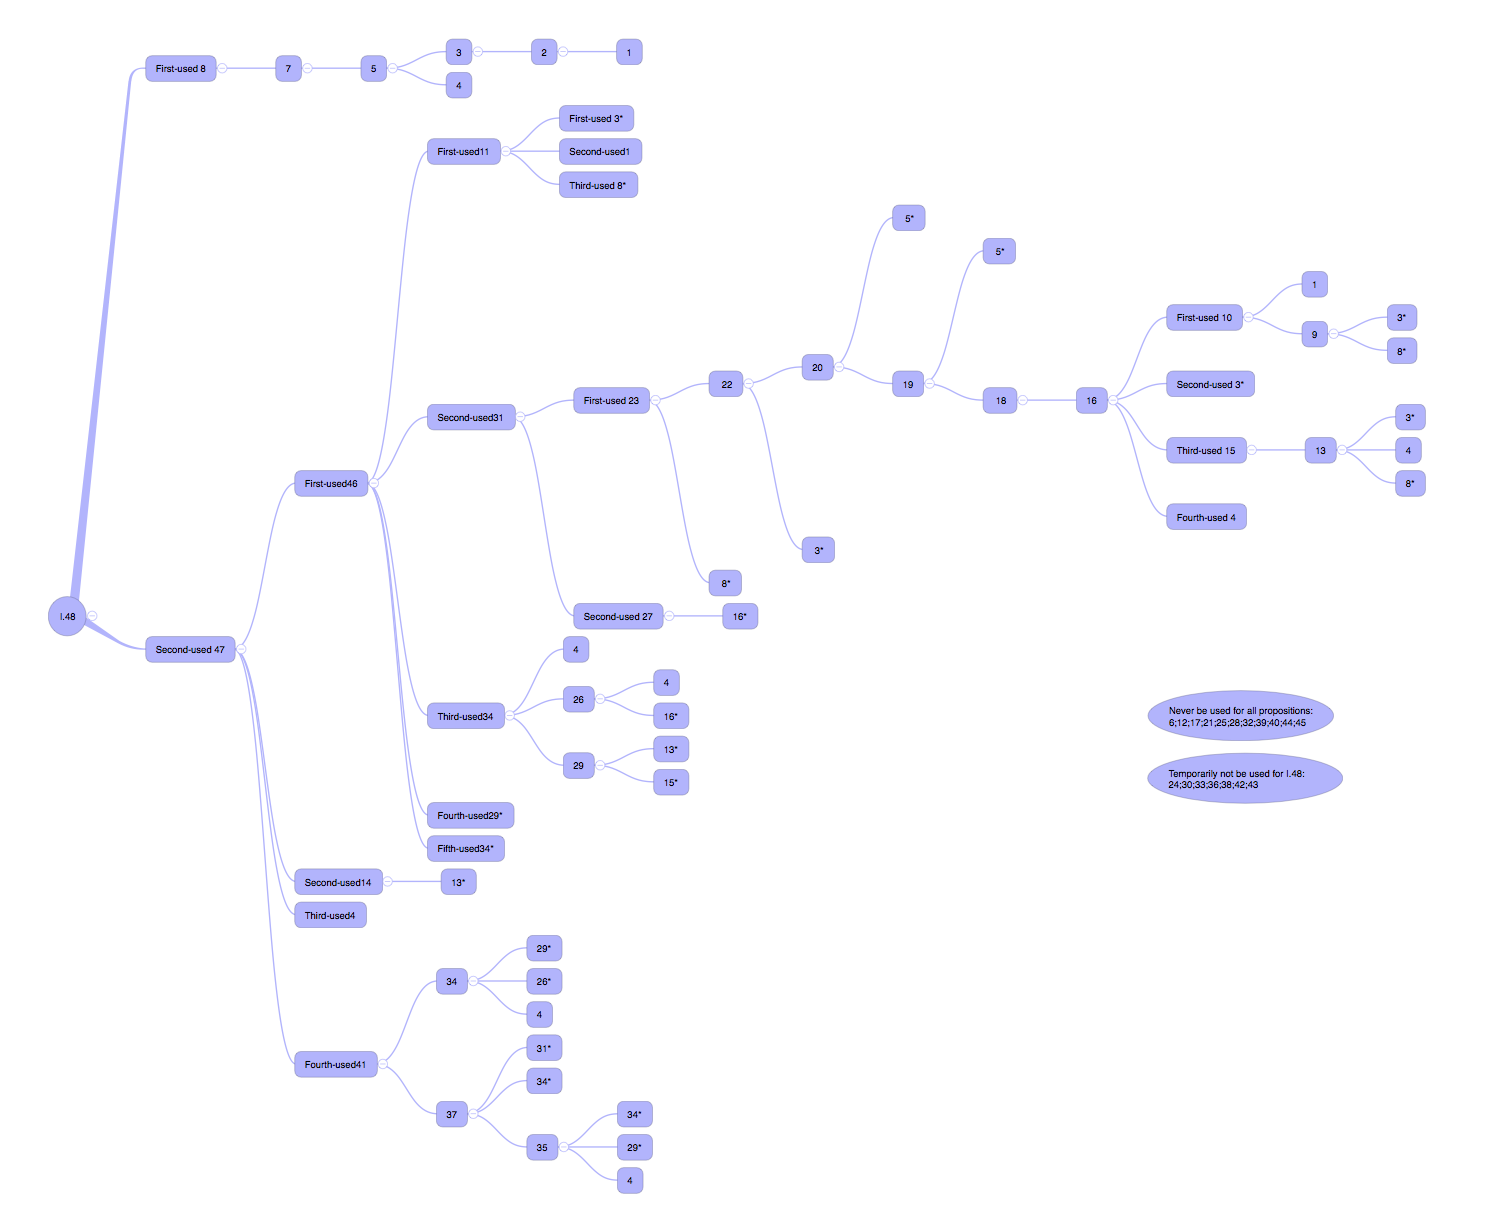
\includegraphics[width=1\linewidth]{./image/18-prop48-image15}

以第一卷的结尾命题48倒着通过引用的内容进行展开,可以看到逻辑发展的脉络。主线自然是最长的那一条,且这条最长的证明线的尽头是命题一。其它不同的证明线在四十七的证明中也有自己存在的目的。
做这个脉络整理的原因是想展示出西方勾股定理从零开始到证明完成中间的过程,是怎样一环扣一环推进的。而中国古代的证明方法则非常不同,以刘徽的割补术为例。割补术的特点是它从实际的角度出发,完全省略了抽象世界的构建,因此它不需要一系列证明定义的铺垫,它直接就给定图形,用拼凑的方法来证明。并且它假定了视觉认知的意义,认为可以直接认定``入''和``出''不同部分的相等性,而无需给出证明。中国古代的方法,相对而言实用性很高,易于理解,和动手能力相关。如果我们读《九章算术》就会发现,整本书从算田地的面积这种生活实用题出发,这其实会引发一个思考,西方的证明式的数学和中国古代的应用类数学,在今天都被称为数学,但是它们真的是在谈论同一个事情么???

\hypertarget{ux547dux9898ux56dbux5341ux516b}{%
\section{命题四十八}\label{ux547dux9898ux56dbux5341ux516b}}

\textbf{如果在一个三角形中,一边上的正方形等于剩余两边上正方形之和,那么剩余两边所夹角为直角。}

命题四十八是整卷书的收尾,其实就是命题四十七的反证明,将条件和结论进行了一个置换,如果命题四十七中证出的某某性质存在,则某某条件也必定满足。也因此在我们以四十八为起点整理整卷书的脉络的时候会发现,核心落在四十七的证明中。四十八,更如同是欧几里得习惯的一个呈现,当完成一个重要证明时,将相反的,相关的,延伸性质的还有再创造的相关证明一并给出。

至此,第一卷书的四十八道命题也就全都看完了。

  \bibliography{book.bib,packages.bib}

\end{document}
